\vspace{1.5cm}

\clearpage

\subsubsection{Punto de reposo hallado por simulación}

En la figura~\figref{fig:fig_simulated_qpoint} se muestra lo hallado por simulación para el circuito. Vemos una gran similitud con los valores calculados anteriormente, figura~\figref{fig:fig_calculated_qpoint}, aunque hubo que cambiar el valor de $PS_{401}$ con respecto al calculado para acercarnos lo más posible a $0 \si[per-mode=symbol]{\volt}$ en la salida, y también se tuvo que cambiar el valor de $PS_{402_{A}}$ y $PS_{402_{B}}$ para asegurar $10 \si[per-mode=symbol]{\milli\ampere}$ en los colectores de $Q_{407}$ y $Q_{408}$.


\begin{figure}[H] %htb
\begin{center}
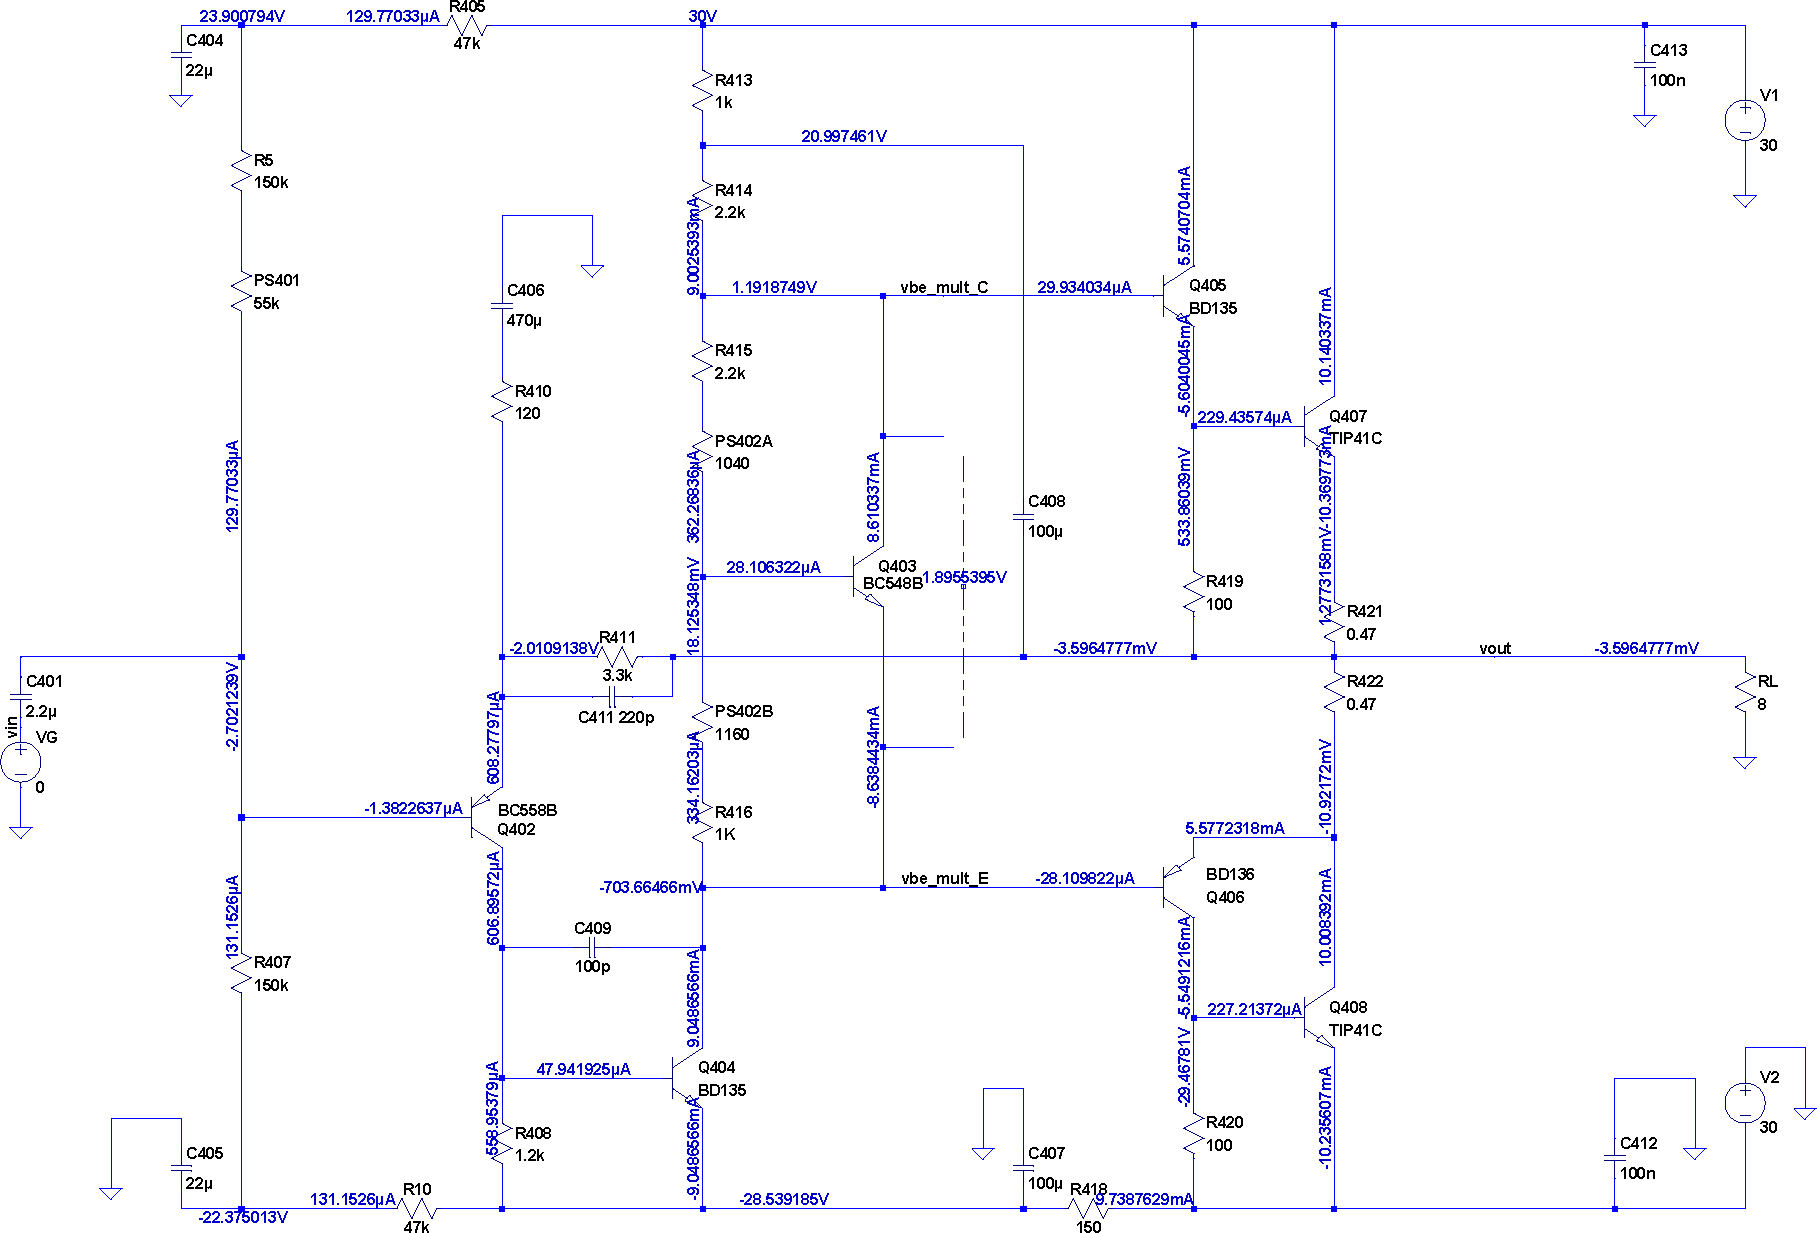
\includegraphics[width=0.9 \textwidth, angle=90]{./img/circuitos_usados/P1_P11a_qpoint.png}
\caption{\label{fig:fig_simulated_qpoint}\footnotesize{Punto de reposo del circuito hallado por simulación.}}
\end{center}
\end{figure}


\clearpage

\subsubsection{Impedancia de entrada hallada por simulación}

En la figura~\figref{fig:fig_simulated_zi} se muestra lo obtenido al simular para obtener la impedancia de entrada, el valor a frecuencias medias $86.02 \si[per-mode=symbol]{\kilo\ohm}$ se acerca bastante al valor calculado en la sección~\sectref{calculated_zi}, se había calculado $85.3 \si[per-mode=symbol]{\kilo\ohm}$.


\begin{figure}[H] %htb
\begin{center}
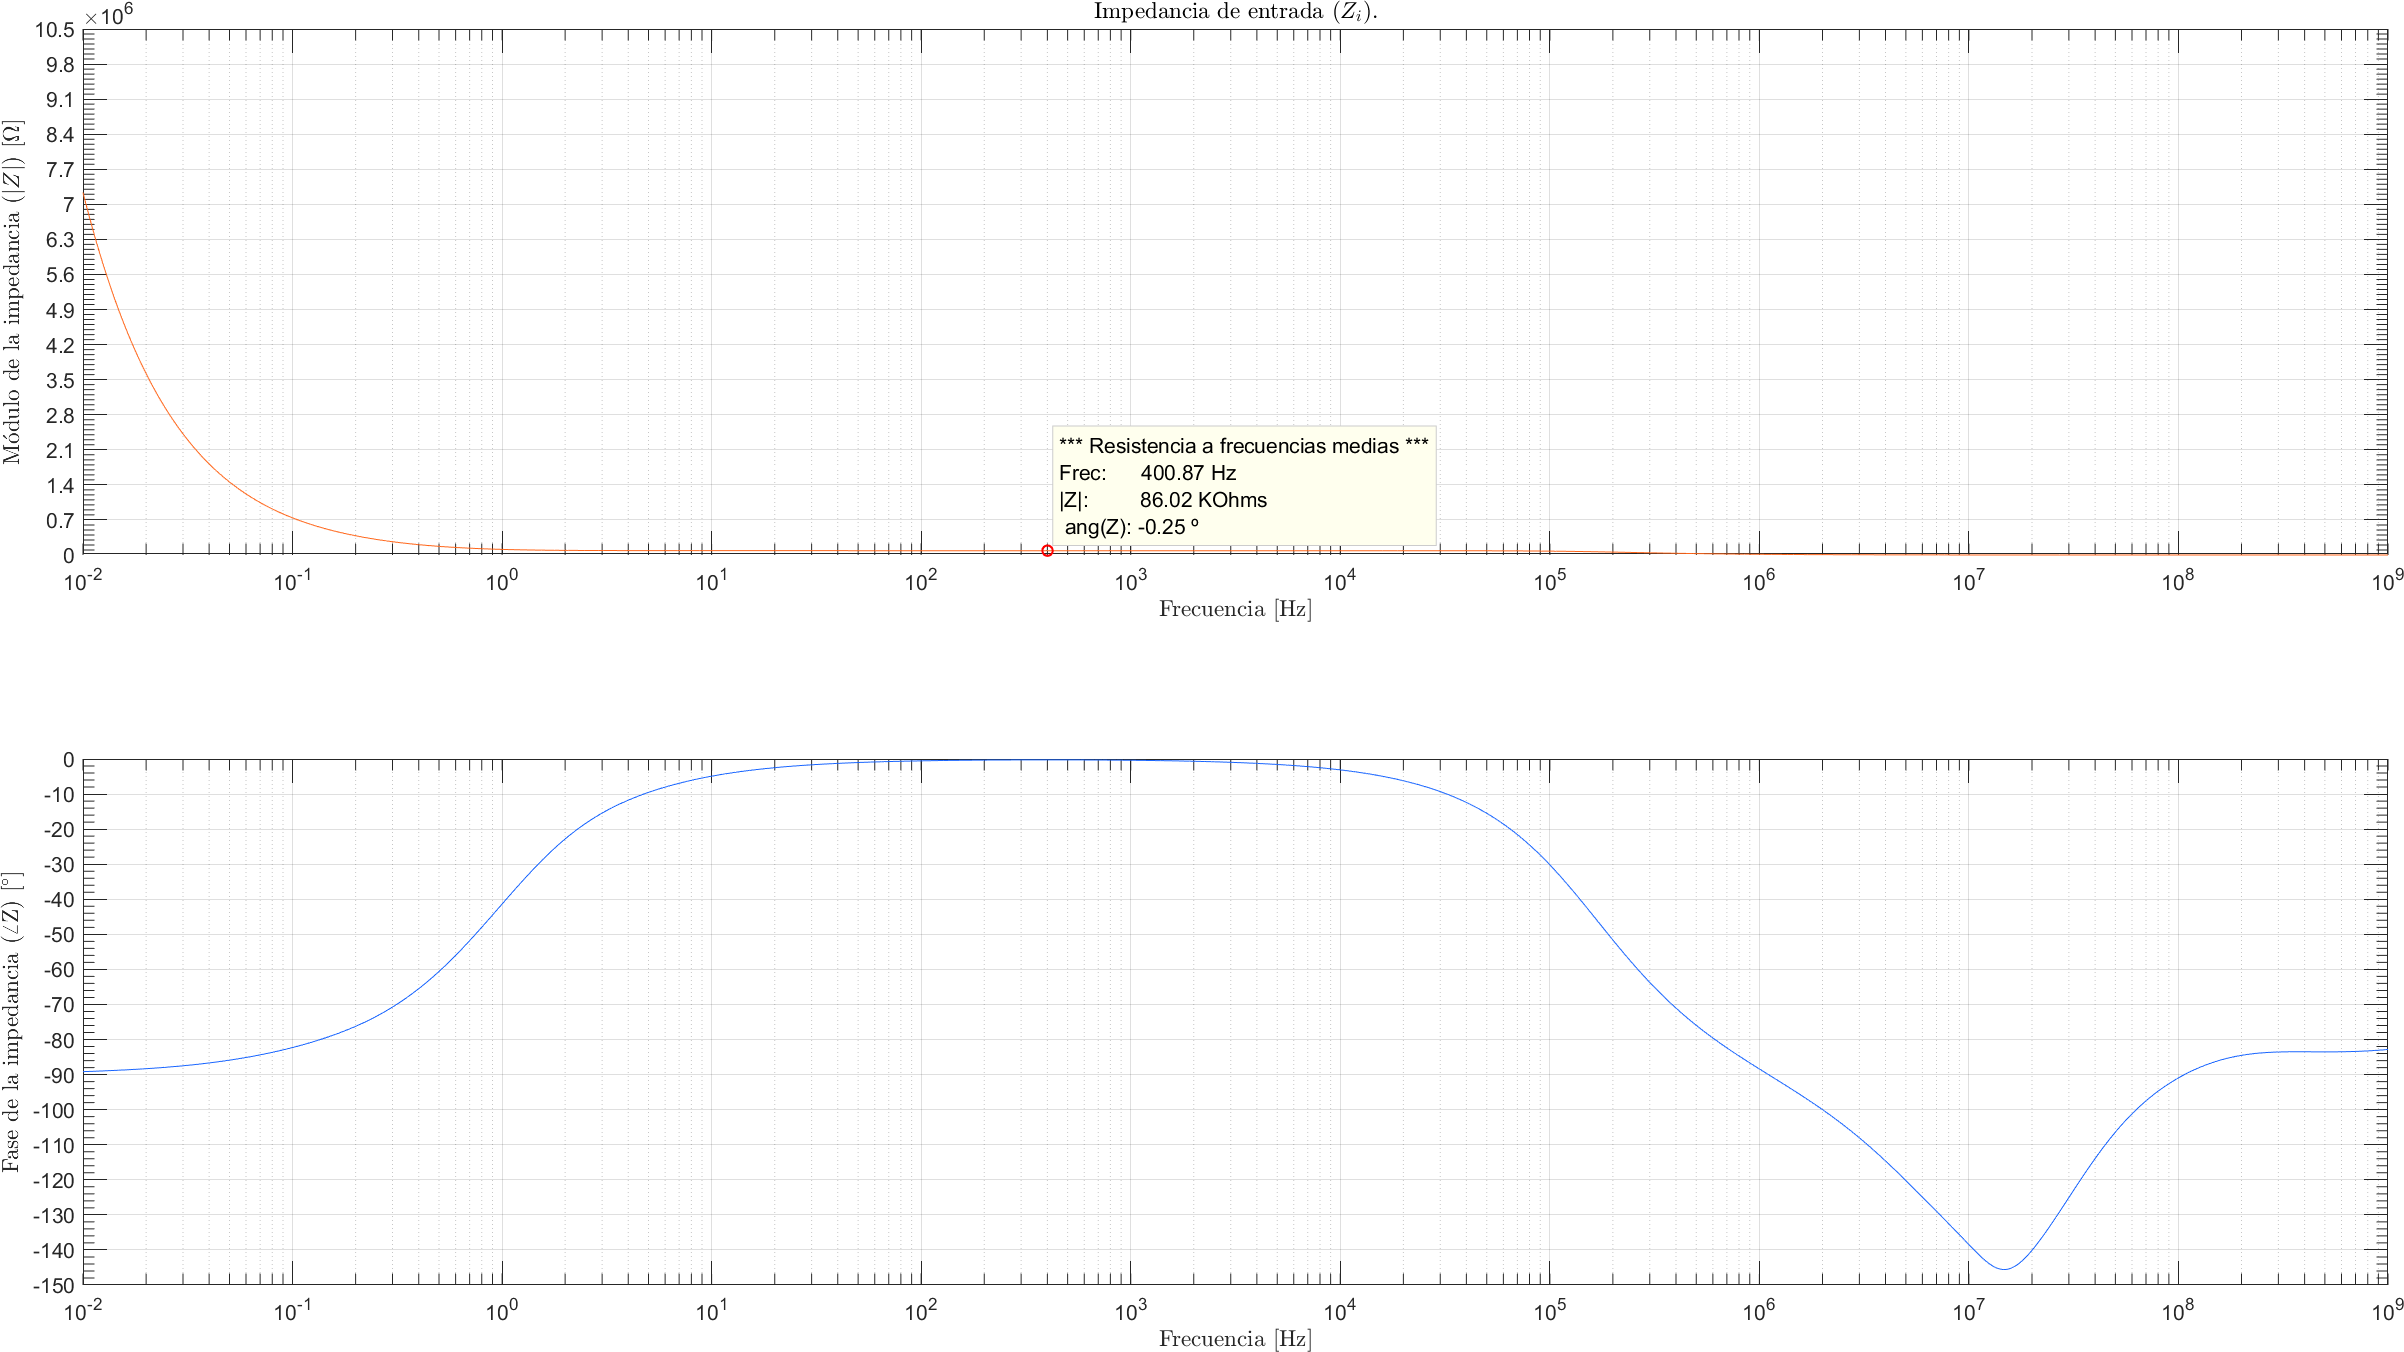
\includegraphics[width=0.9 \textwidth, angle=90]{./img/puntos/P11b_Ri.png}
\caption{\label{fig:fig_simulated_zi}\footnotesize{Impedancia de entrada hallada por simulación.}}
\end{center}
\end{figure}



\clearpage

\subsubsection{Impedancia de salida hallada por simulación}

En la figura~\figref{fig:fig_simulated_zo} se muestra lo obtenido al simular para obtener la impedancia de salida, el valor a frecuencias medias $17.58 \si[per-mode=symbol]{\milli\ohm}$ se aparta un poco del valor calculado en la sección~\sectref{calculated_zo}, se había calculado $29.6 \si[per-mode=symbol]{\milli\ohm}$, pero por lo dicho en dicha sección acerca del cálculo de la impedancia de salida a lazo abierto y por la fuerte dependencia del valor con la ganancia de lazo, que se calcula en forma aproximada, era esperable la diferencia.


\begin{figure}[H] %htb
\begin{center}
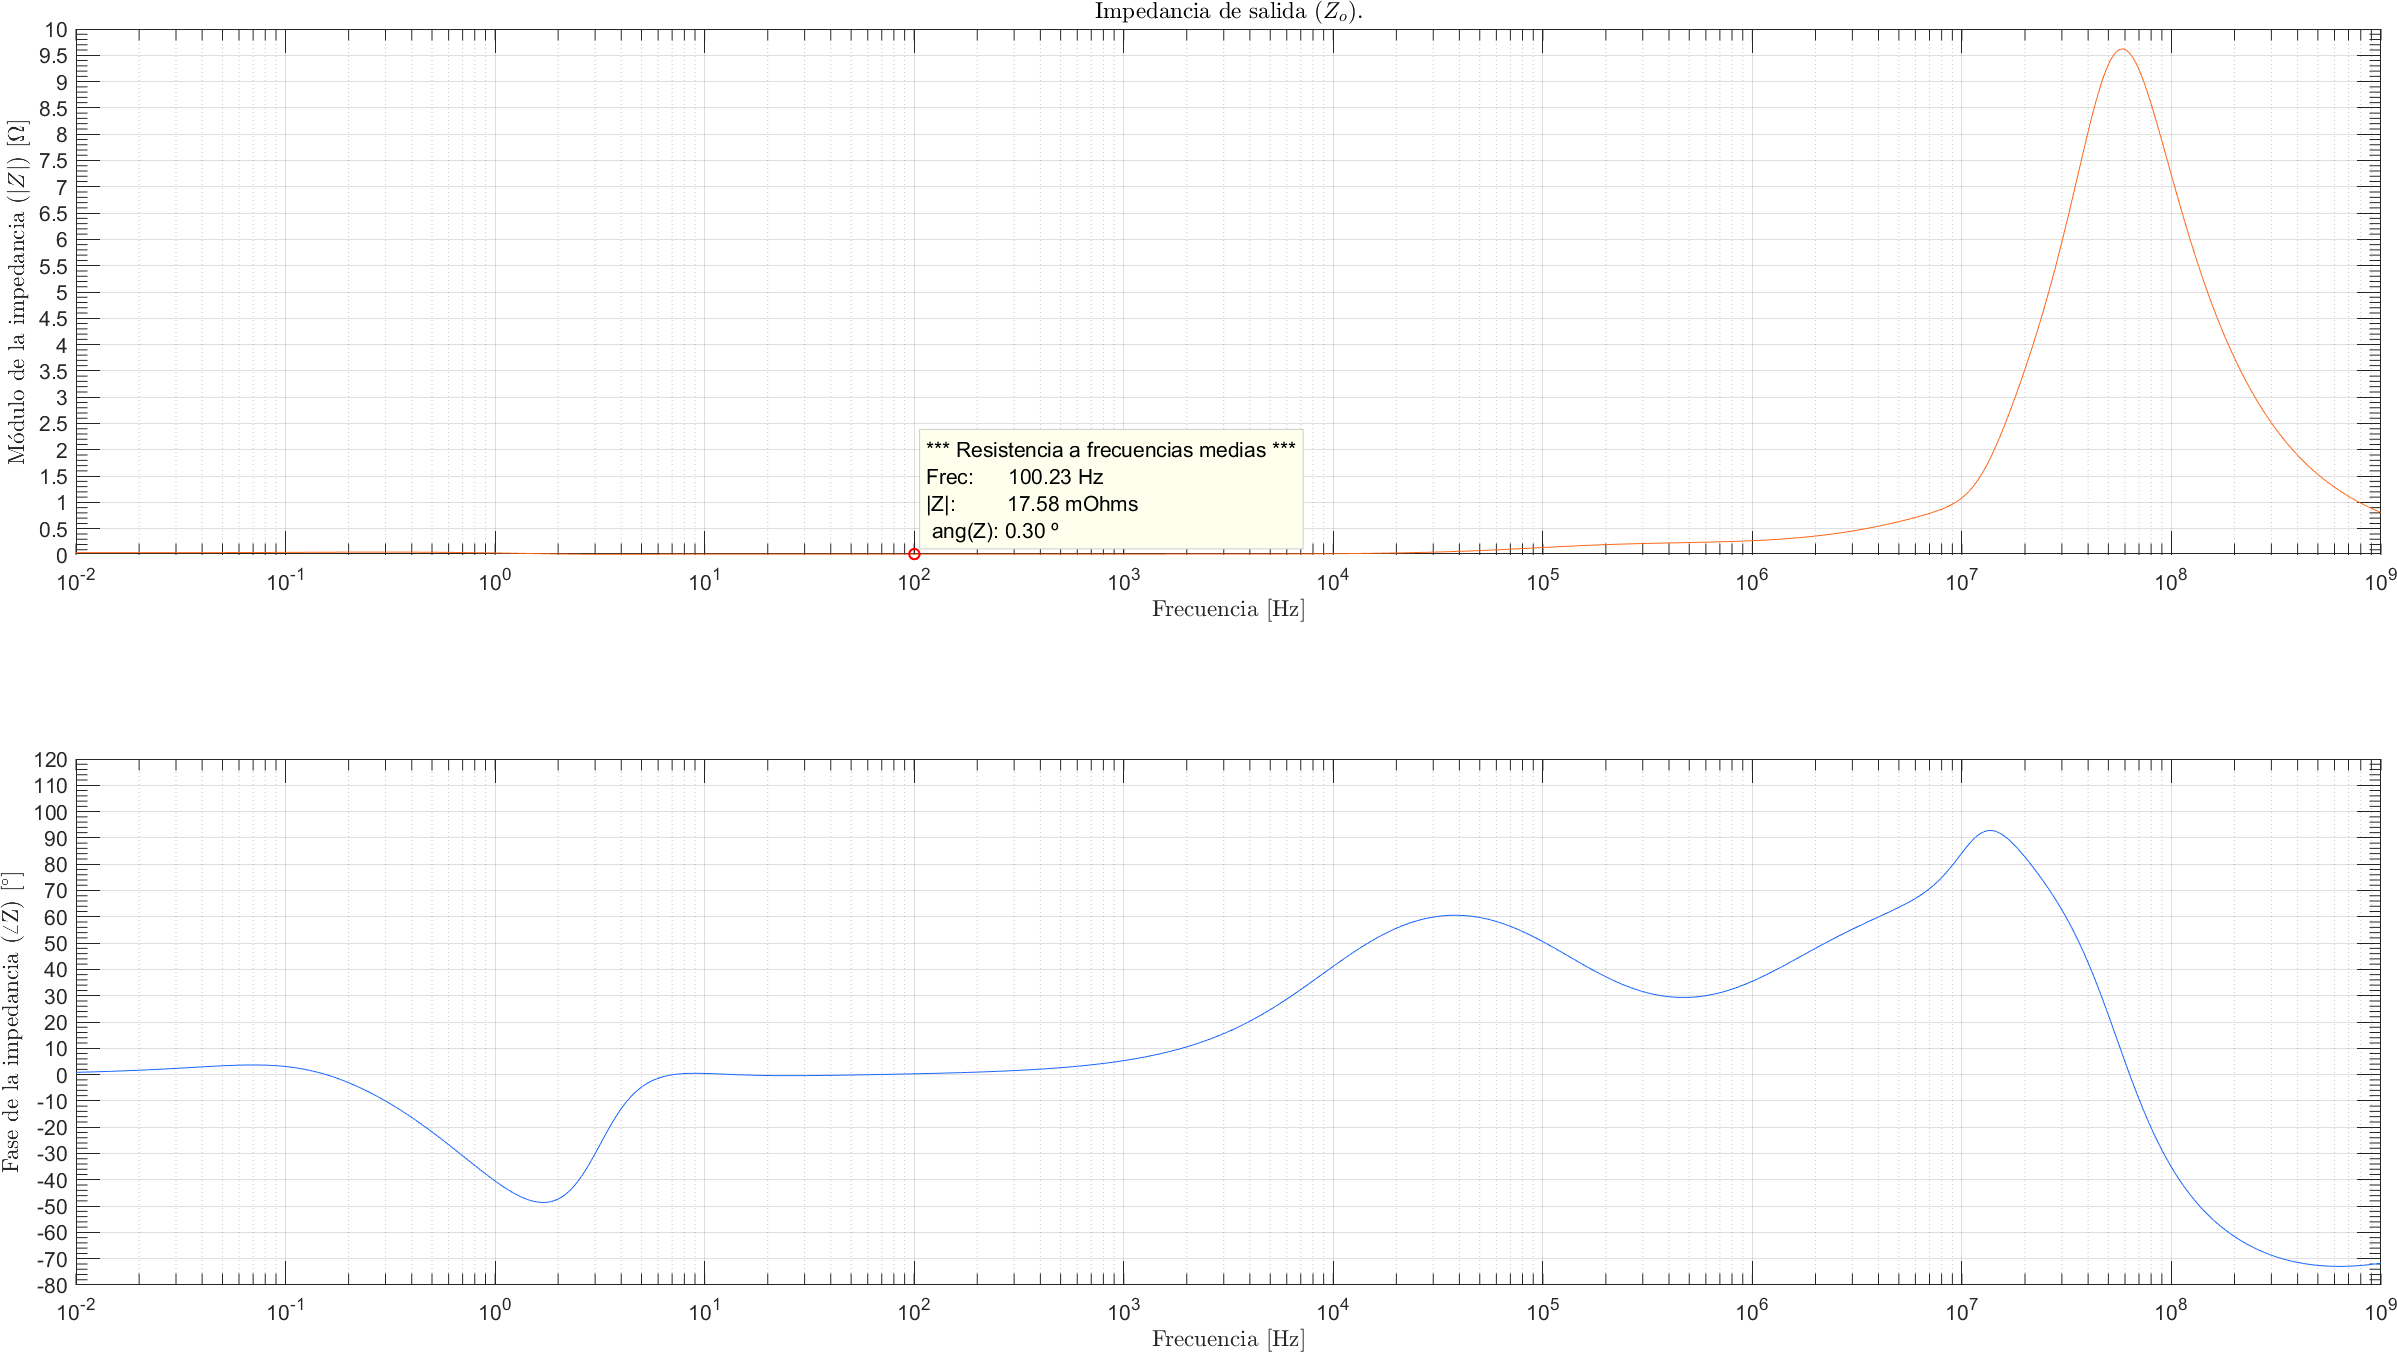
\includegraphics[width=0.9 \textwidth, angle=90]{./img/puntos/P11c_Ro.png}
\caption{\label{fig:fig_simulated_zo}\footnotesize{Impedancia de salida hallada por simulación.}}
\end{center}
\end{figure}



\clearpage

\subsubsection{Respuesta en frecuencia para $1 \si[per-mode=symbol]{\watt}$ sobre la carga}

En la figura~\figref{fig:fig_RF_1W} se muestra lo obtenido al simular para obtener la respuesta en frecuencia a $1 \si[per-mode=symbol]{\watt}$ de potencia sobre la carga, en la misma se puede ver el valor del ancho de banda encontrado, $129.55 \si[per-mode=symbol]{\kilo\hertz}$.

\begin{figure}[H] %htb
\begin{center}
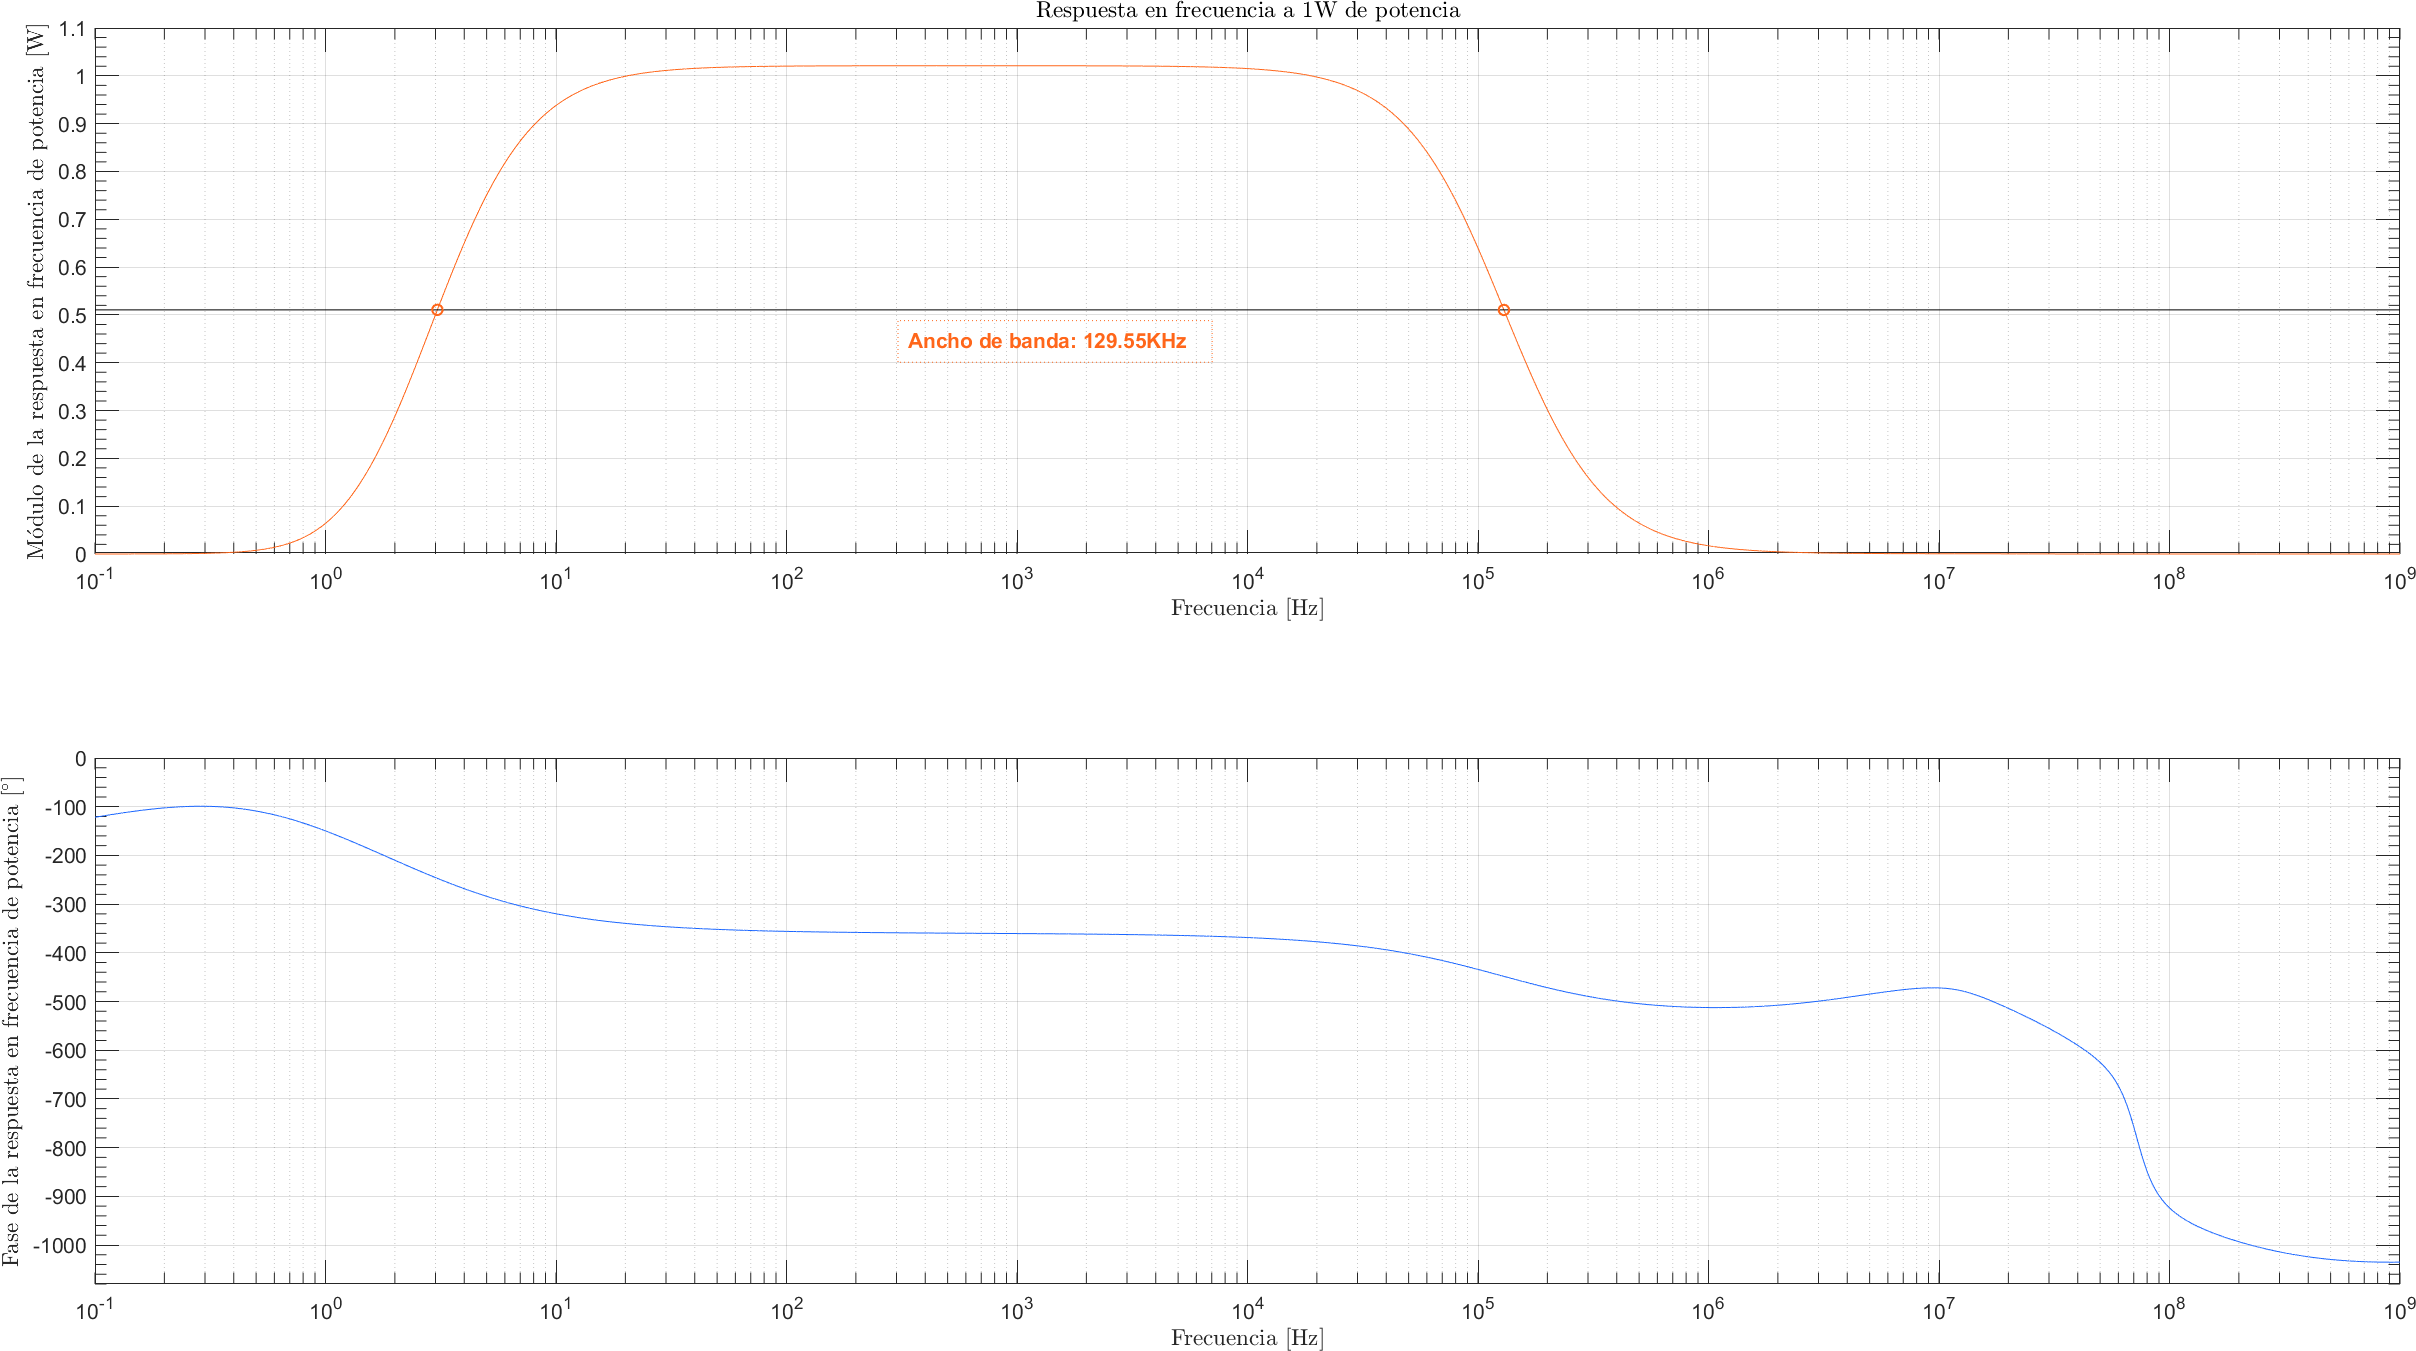
\includegraphics[width=0.9 \textwidth, angle=90]{./img/puntos/P11d_RF_1W.png}
\caption{\label{fig:fig_RF_1W}\footnotesize{Respuesta en frecuencia para $1 \si[per-mode=symbol]{\watt}$ sobre la carga.}}
\end{center}
\end{figure}


\clearpage

\subsubsection{Ancho de banda de potencia, a máxima potencia sobre la carga}

En la figura~\figref{fig:fig_RF_MAX_POWER} se muestra lo obtenido al simular para obtener la respuesta en frecuencia a $1 \si[per-mode=symbol]{\watt}$ de potencia sobre la carga, en la misma se puede ver el valor del ancho de banda encontrado, $129.55 \si[per-mode=symbol]{\kilo\hertz}$, idéntico que para el caso de $1 \si[per-mode=symbol]{\watt}$ .

\begin{figure}[H] %htb
\begin{center}
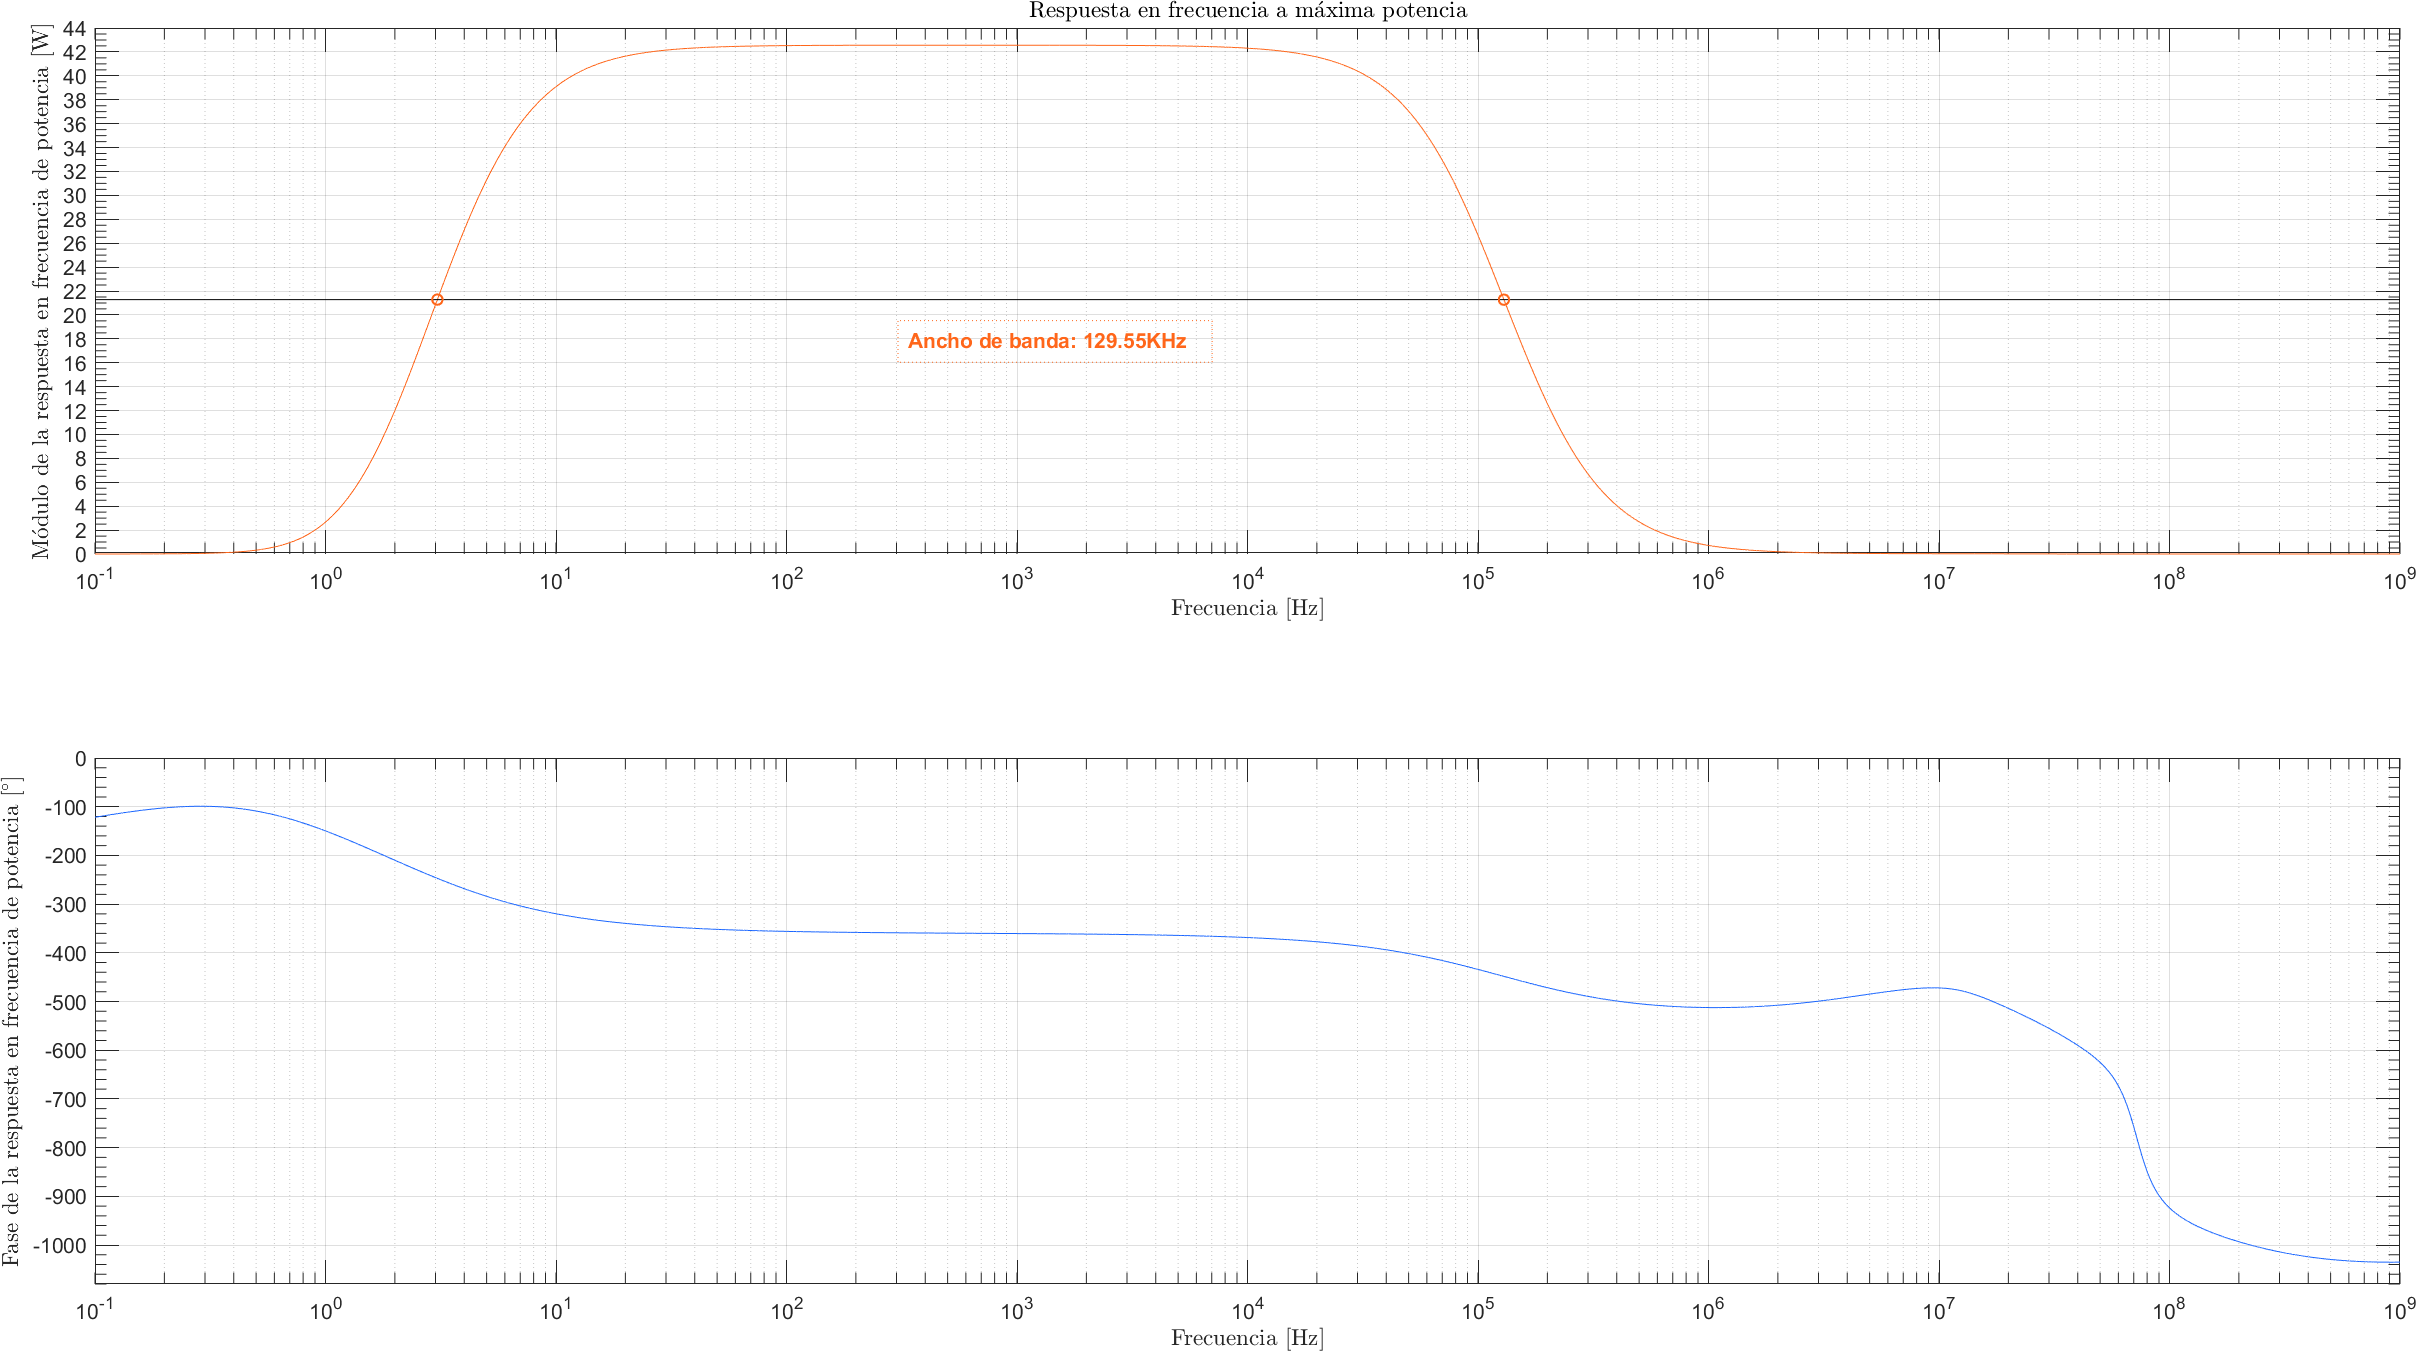
\includegraphics[width=0.9 \textwidth, angle=90]{./img/puntos/P11e_Power_BW.png}
\caption{\label{fig:fig_RF_MAX_POWER}\footnotesize{Respuesta en frecuencia para máxima potencia sobre la carga.}}
\end{center}
\end{figure}


\clearpage

\subsubsection{Respuesta al escalón en pequeña señal}

En la figura~\figref{fig:fig_step_small_signal} se muestra lo obtenido al simular para obtener la respuesta al escalón en pequeña señal, se limitó la salida a un valor de $1 \si[per-mode=symbol]{\volt}$ de pico. La respuesta tiene la forma esperada para un amplificador con acoples capacitivos.

\begin{figure}[H] %htb
\begin{center}
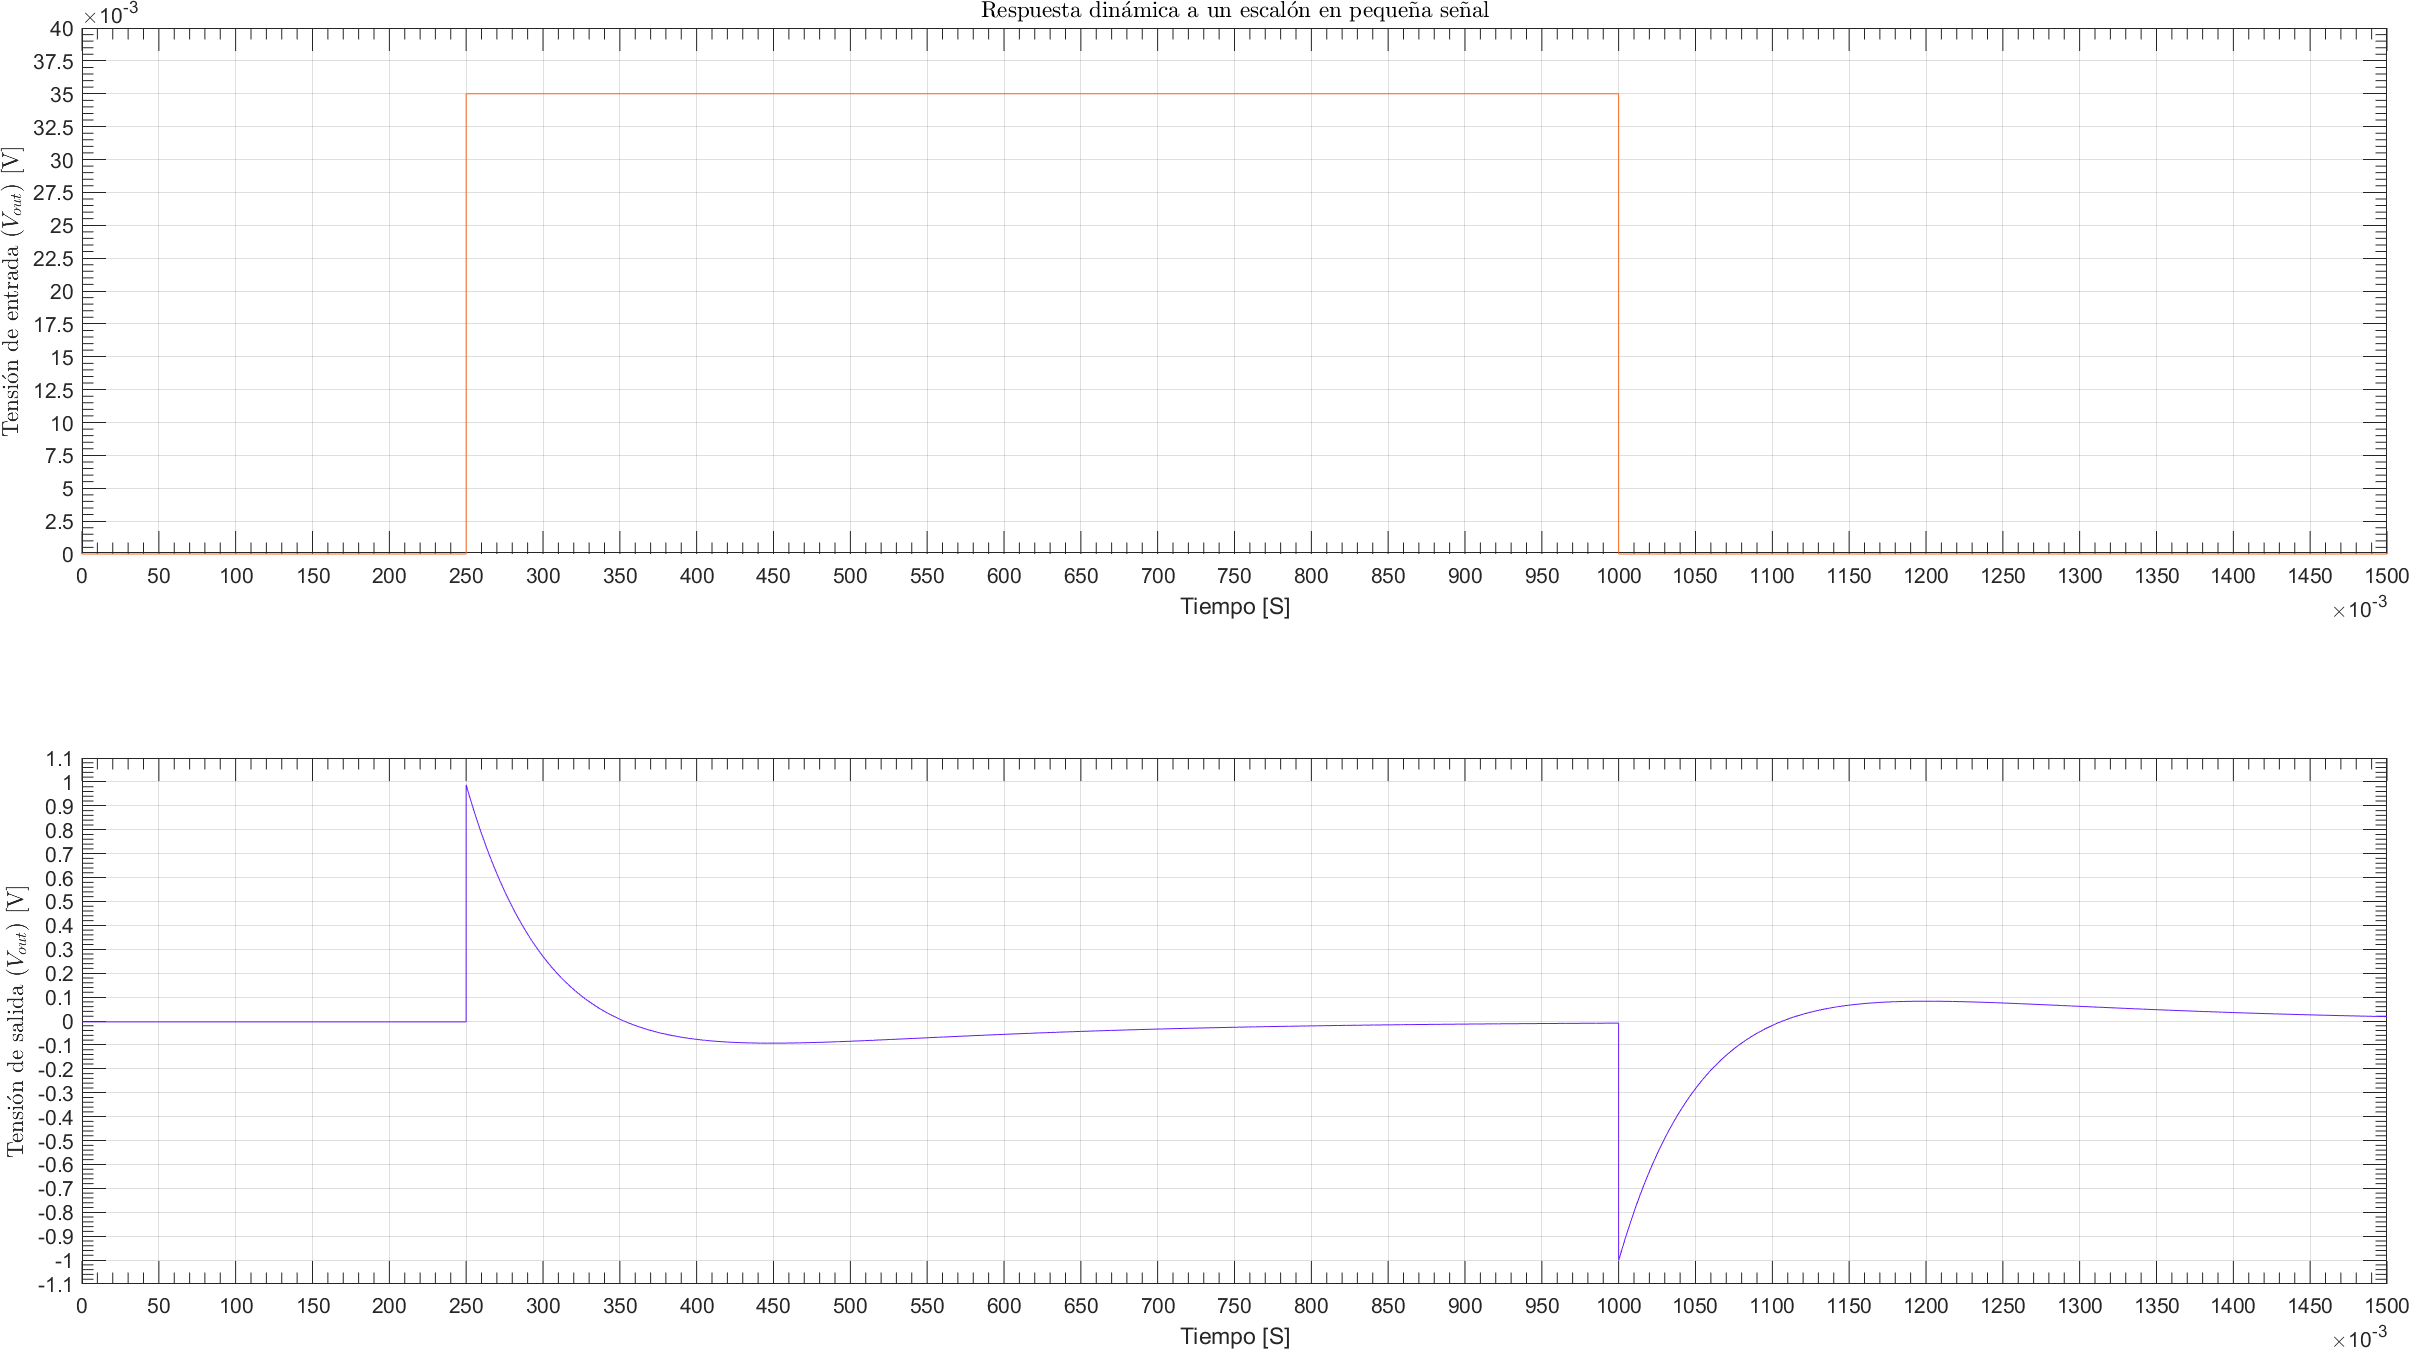
\includegraphics[width=0.9 \textwidth, angle=90]{./img/puntos/P11f_I_step_small_signal.png}
\caption{\label{fig:fig_step_small_signal}\footnotesize{Respuesta al escalón en pequeña señal.}}
\end{center}
\end{figure}


En la figura~\figref{fig:fig_step_small_signal_zoom} se muestra la ampliación del flanco ascendente de la salida, donde se puede apreciar el tiempo de crecimiento, usando la directiva de \textbf{SPICE}, \textit{.measure}, se calculó directamente de la simulación el tiempo de crecimiento entre $10\%$ y $90\%$ y se computó en base a este el ancho de banda del circuito. Se utilizó la expresión que relaciona ancho de banda con el tiempo de crecimiento en un circuito con un solo polo:

\begin{equation}
BW = \frac{0.35}{T_{rise}}
\end{equation}

Se obtuvo:

\begin{equation}
T_{rise} = 2.78 \si[per-mode=symbol]{\micro\second}
\end{equation}


\begin{equation}
\boxed{BW = 125.863 \si[per-mode=symbol]{\kilo\hertz}}
\end{equation}



\begin{figure}[H] %htb
\begin{center}
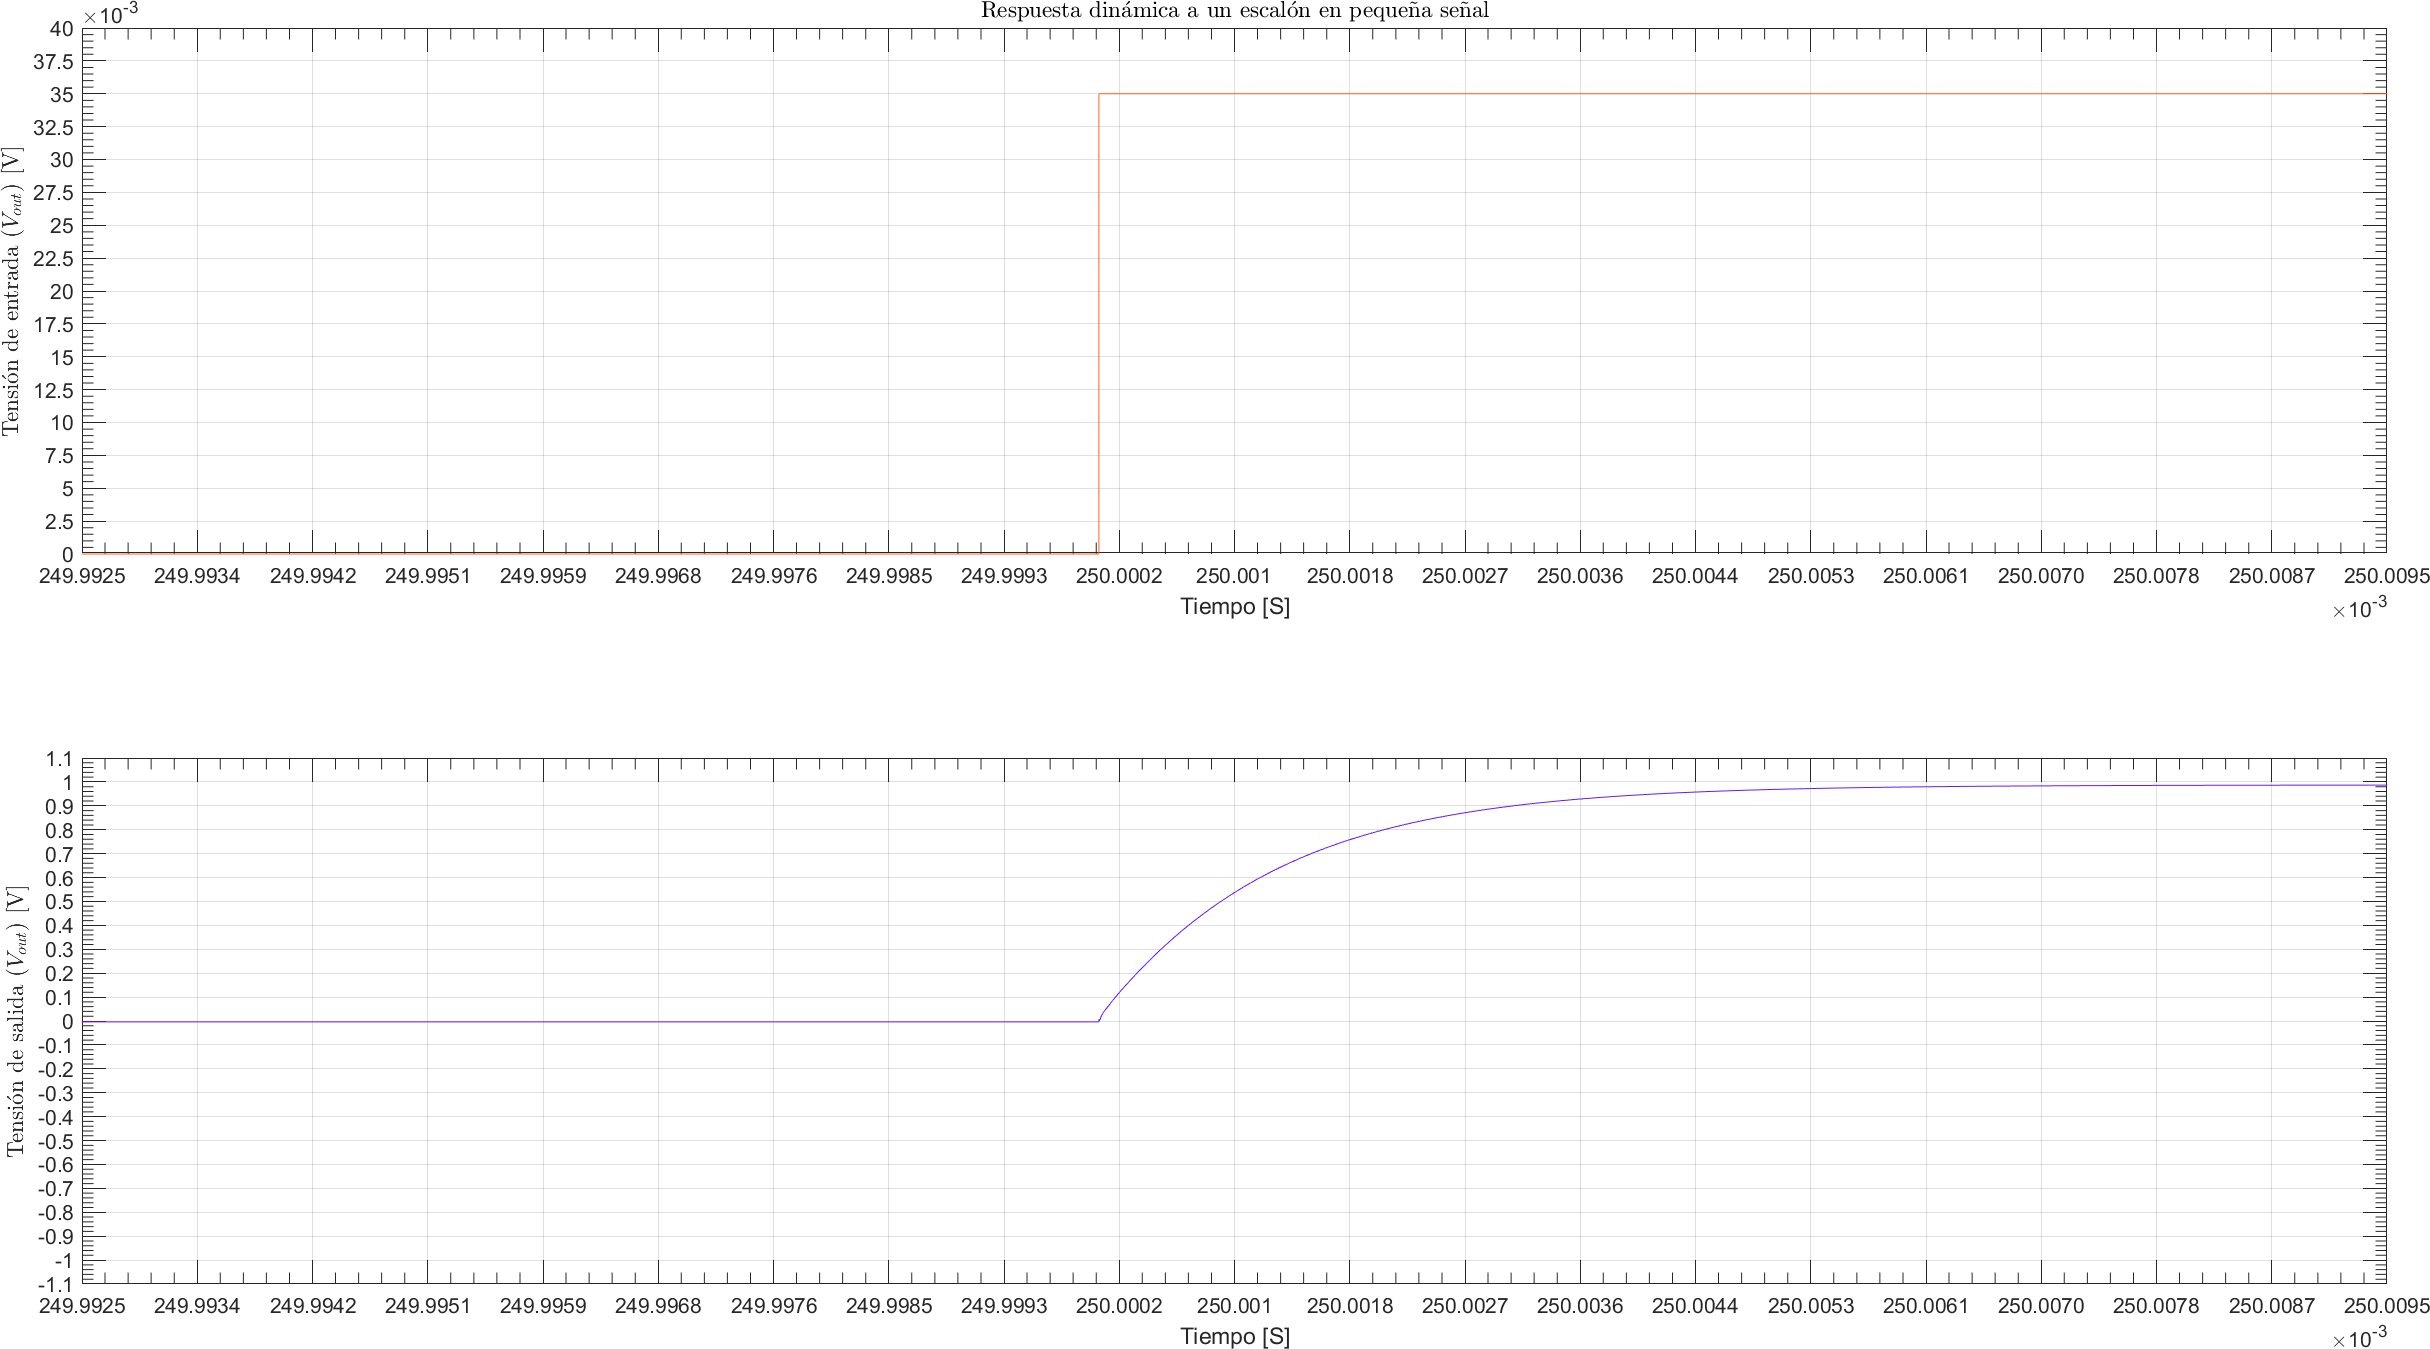
\includegraphics[width=0.9 \textwidth, angle=90]{./img/puntos/P11f_I_step_small_signal_zoom.png}
\caption{\label{fig:fig_step_small_signal_zoom}\footnotesize{Respuesta al escalón en pequeña señal, ampliación del flanco.}}
\end{center}
\end{figure}

\clearpage

\subsubsection{Respuesta al escalón en gran señal}

En la figura~\figref{fig:fig_step_big_signal} se muestra lo obtenido al simular para obtener la respuesta al escalón en gran señal, se llevó la salida a un valor cercano al máximo sin distorsión.

\begin{figure}[H] %htb
\begin{center}
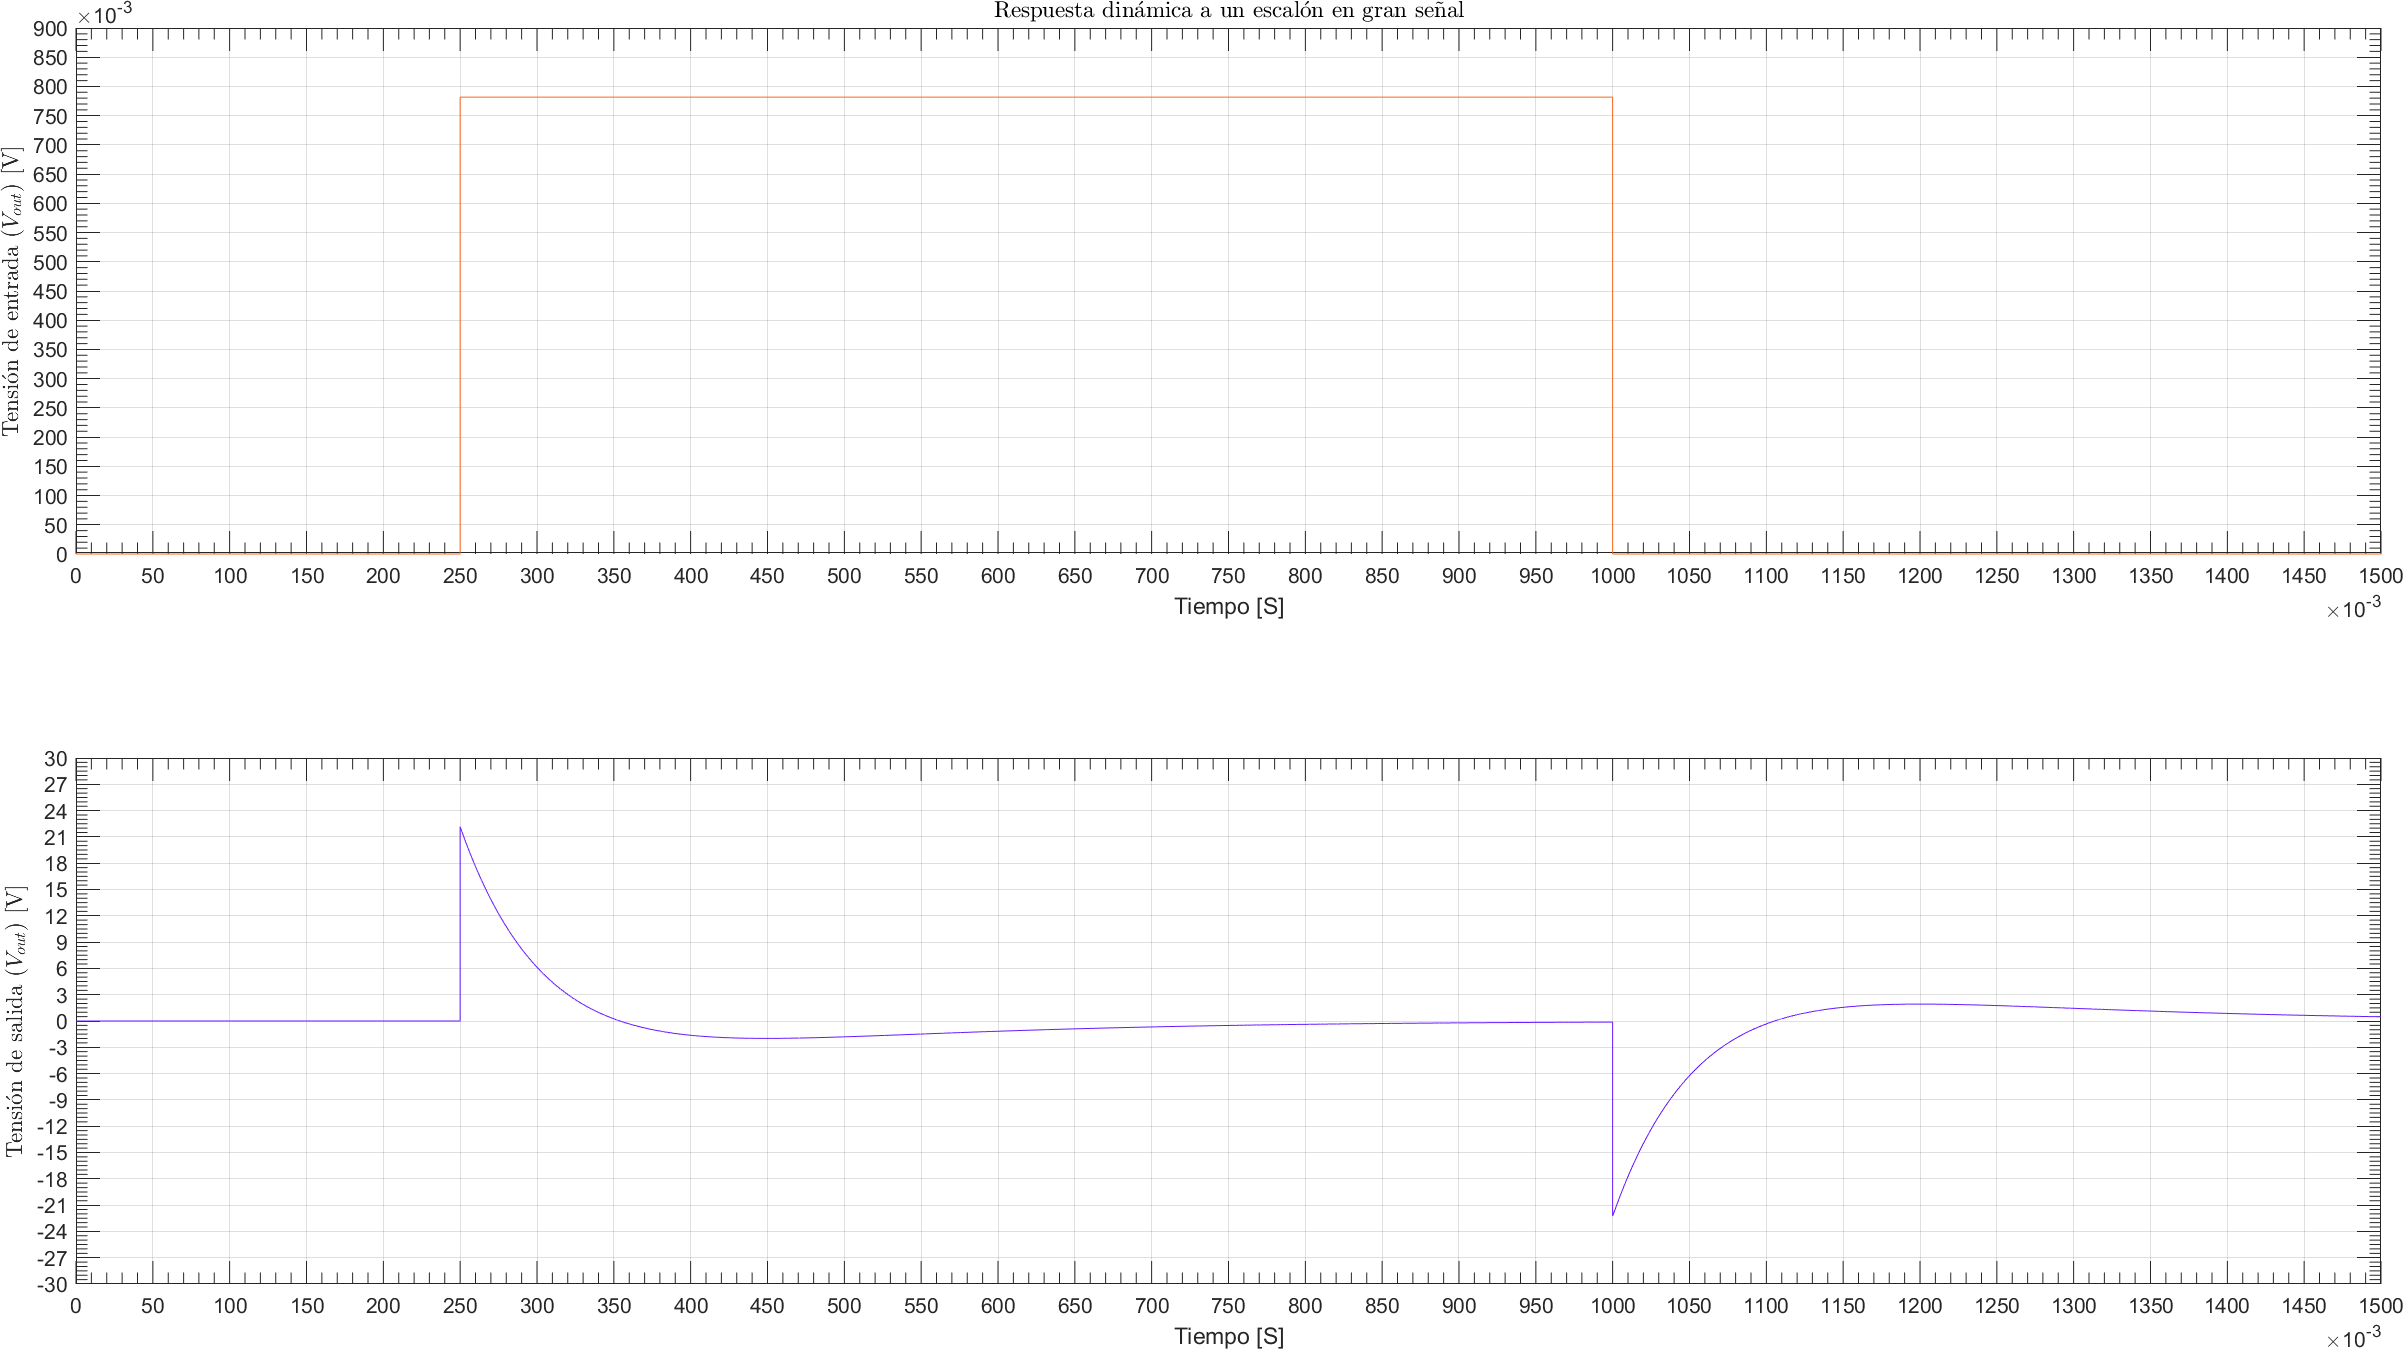
\includegraphics[width=0.9 \textwidth, angle=90]{./img/puntos/P11f_I_step_big_signal.png}
\caption{\label{fig:fig_step_big_signal}\footnotesize{Respuesta al escalón en gran señal.}}
\end{center}
\end{figure}


En la figura~\figref{fig:fig_step_big_signal_zoom} se muestra la ampliación del flanco ascendente de la salida, donde se puede apreciar el tiempo de crecimiento, usando la directiva de \textbf{SPICE}, \textit{.measure}, se calculó directamente de la simulación el \textbf{\quotemarks{slew~rate}}, como la pendiente de subida en el flanco ascendente, se obtuvo:


\begin{equation}
\boxed{SR = 4.39 \si[per-mode=symbol]{\volt\per\micro\second}}
\end{equation}



\begin{figure}[H] %htb
\begin{center}
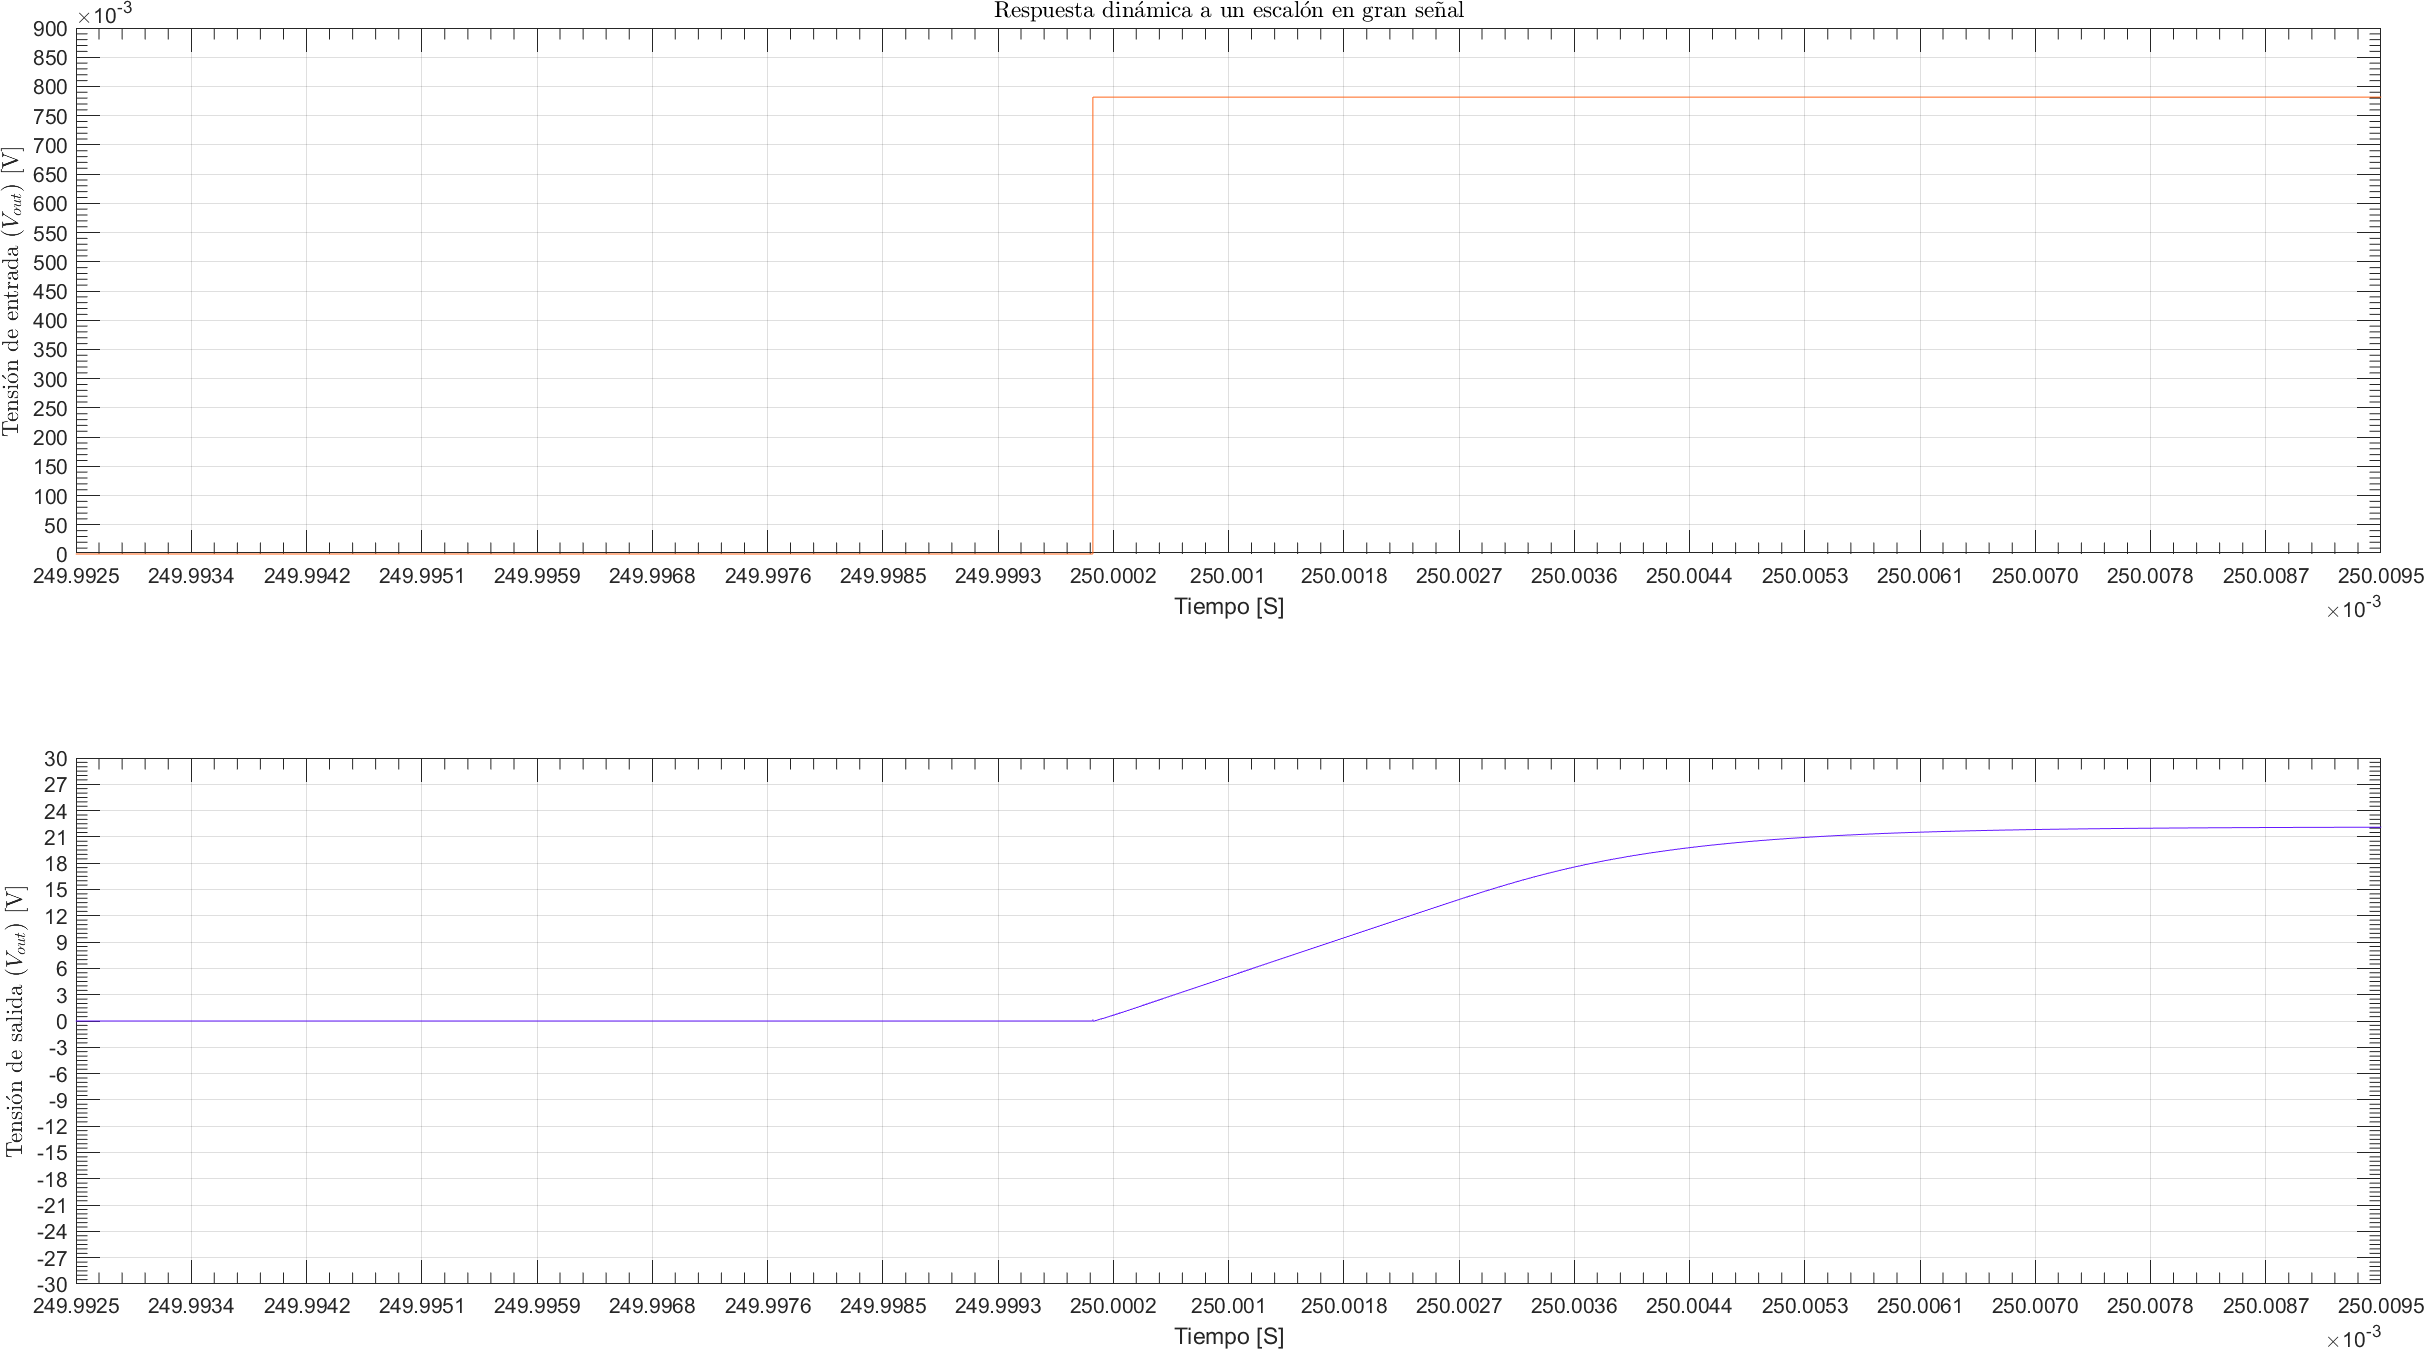
\includegraphics[width=0.9 \textwidth, angle=90]{./img/puntos/P11f_I_step_big_signal_zoom.png}
\caption{\label{fig:fig_step_big_signal_zoom}\footnotesize{Respuesta al escalón en gran señal, ampliación del flanco.}}
\end{center}
\end{figure}

\clearpage


\subsubsection{Margen de fase del amplificador}

En la figura~\figref{fig:fig_phase_margin} se muestra lo obtenido al simular para obtener el margen de fase del circuito, para esta simulación se abrió el lazo de realimentación para la señal y se tomó la respuesta de la cascada del amplificador con la realimentación, en la figura~\figref{fig:fig_loop_gain_circuit}, se puede ver el circuito utilizado para esta simulación. El valor obtenido para el margen de fase es:

\begin{equation}
\boxed{PM = 113.72 \si[per-mode=symbol]{\degree}}
\end{equation}

\begin{figure}[H] %htb
\begin{center}
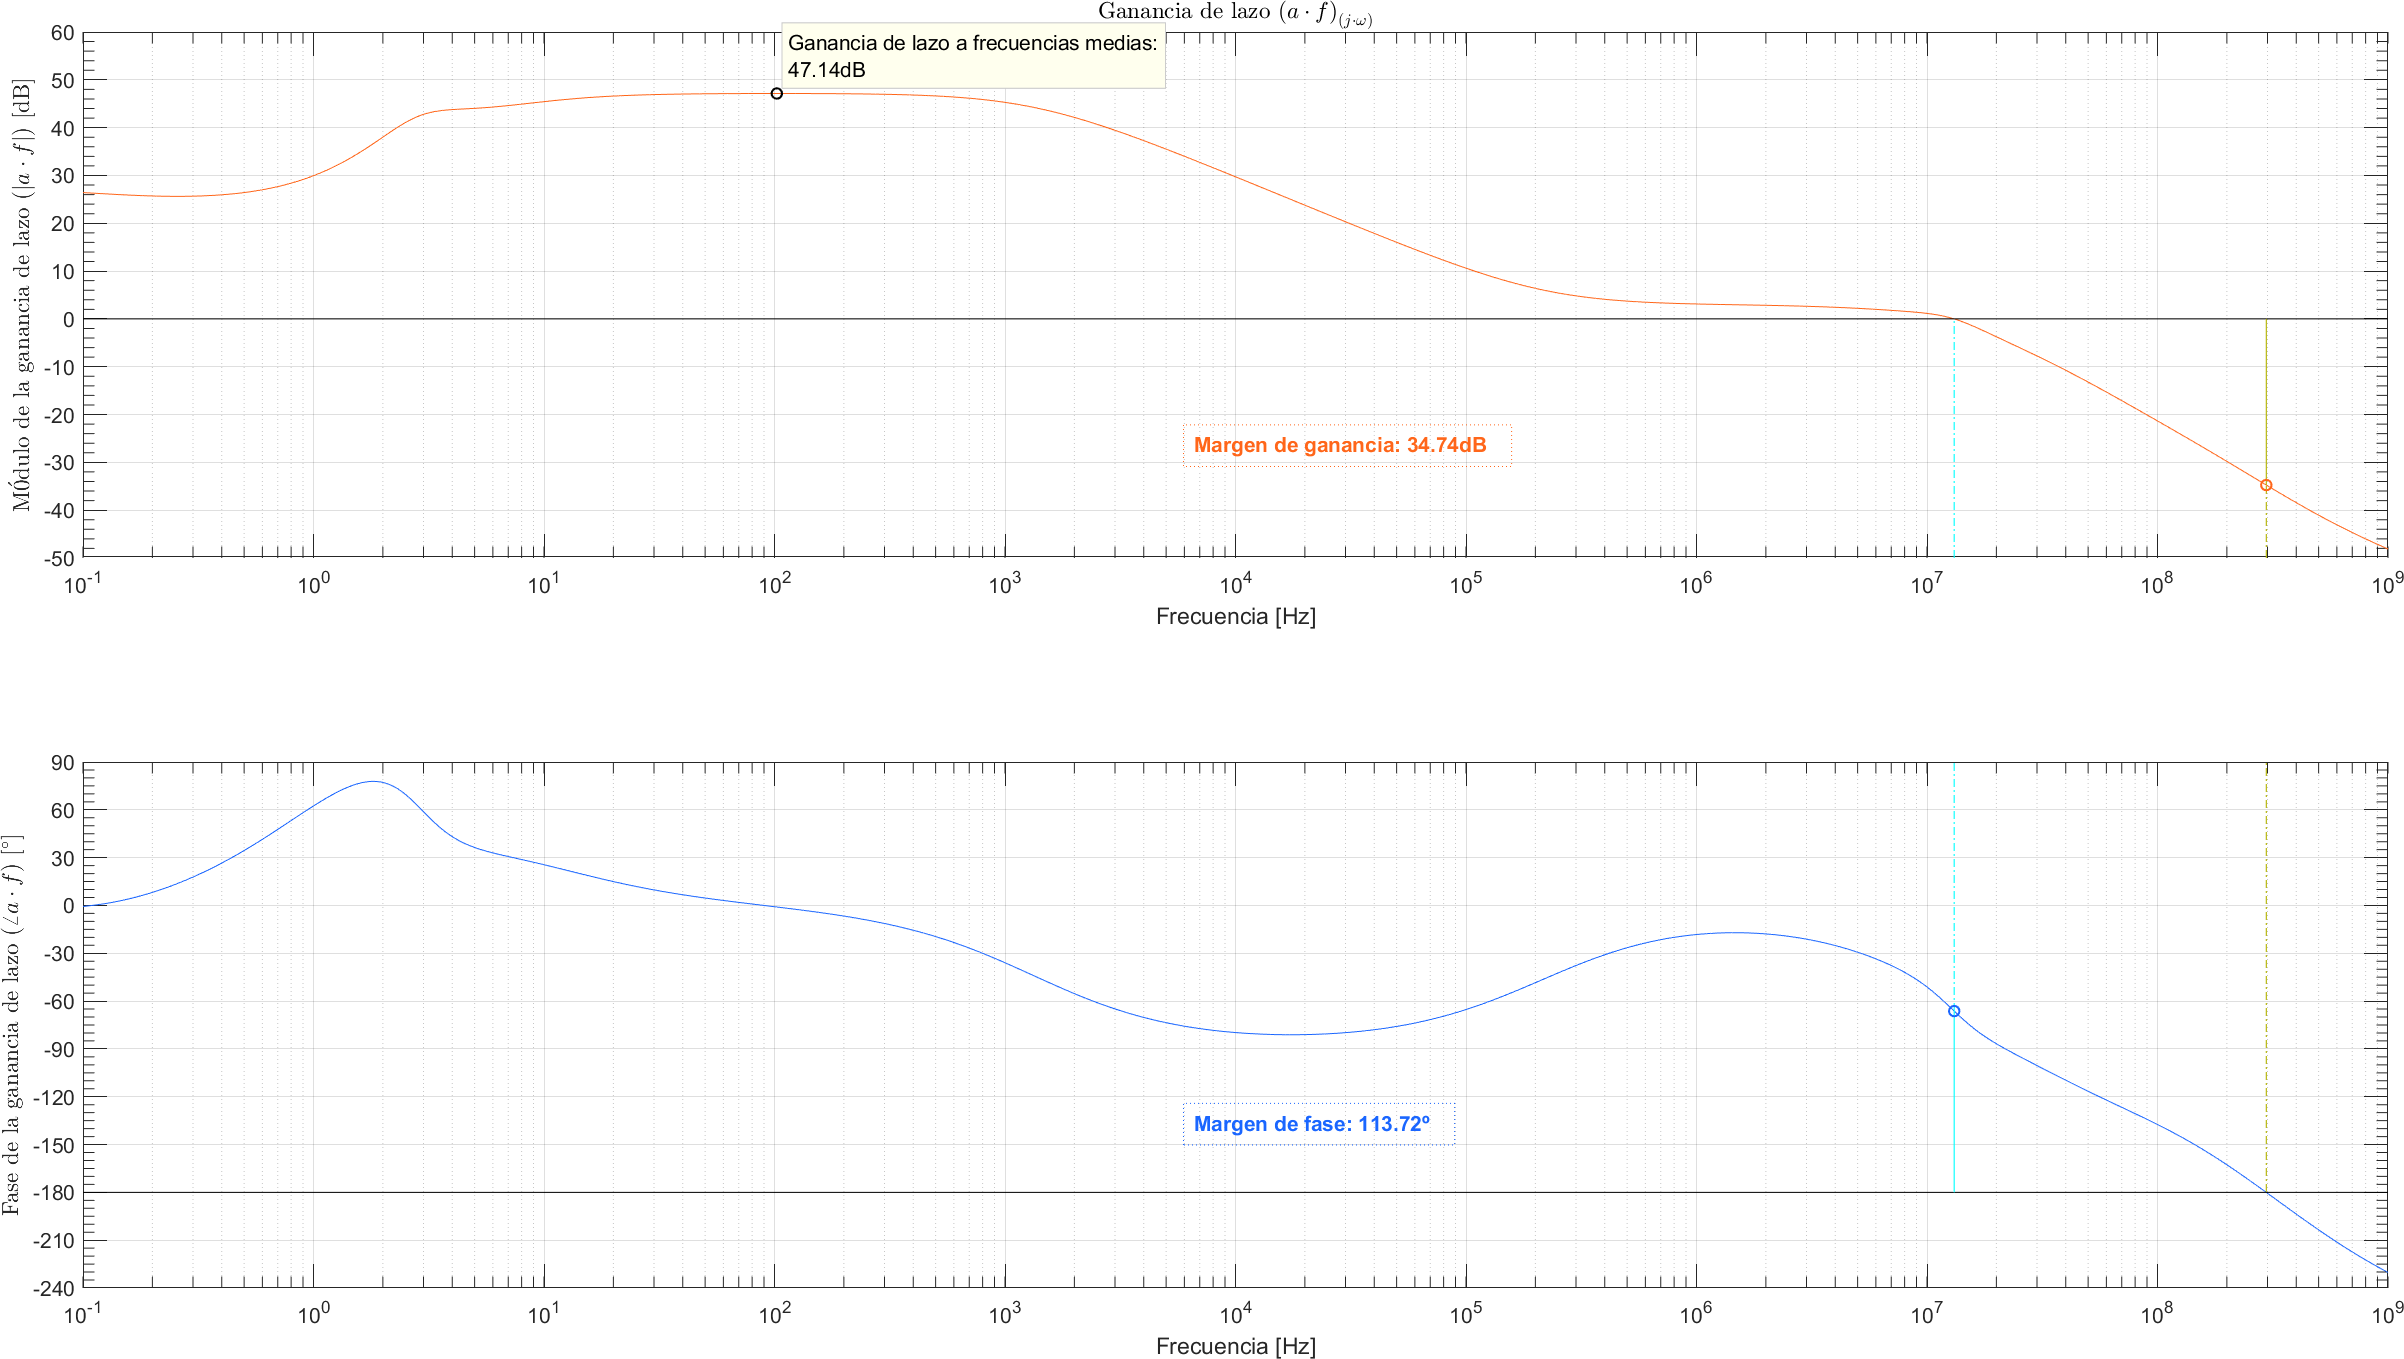
\includegraphics[width=0.9 \textwidth, angle=90]{./img/puntos/P11g_phase_margin.png}
\caption{\label{fig:fig_phase_margin}\footnotesize{Margen de fase.}}
\end{center}
\end{figure}

\begin{figure}[H] %htb
\begin{center}
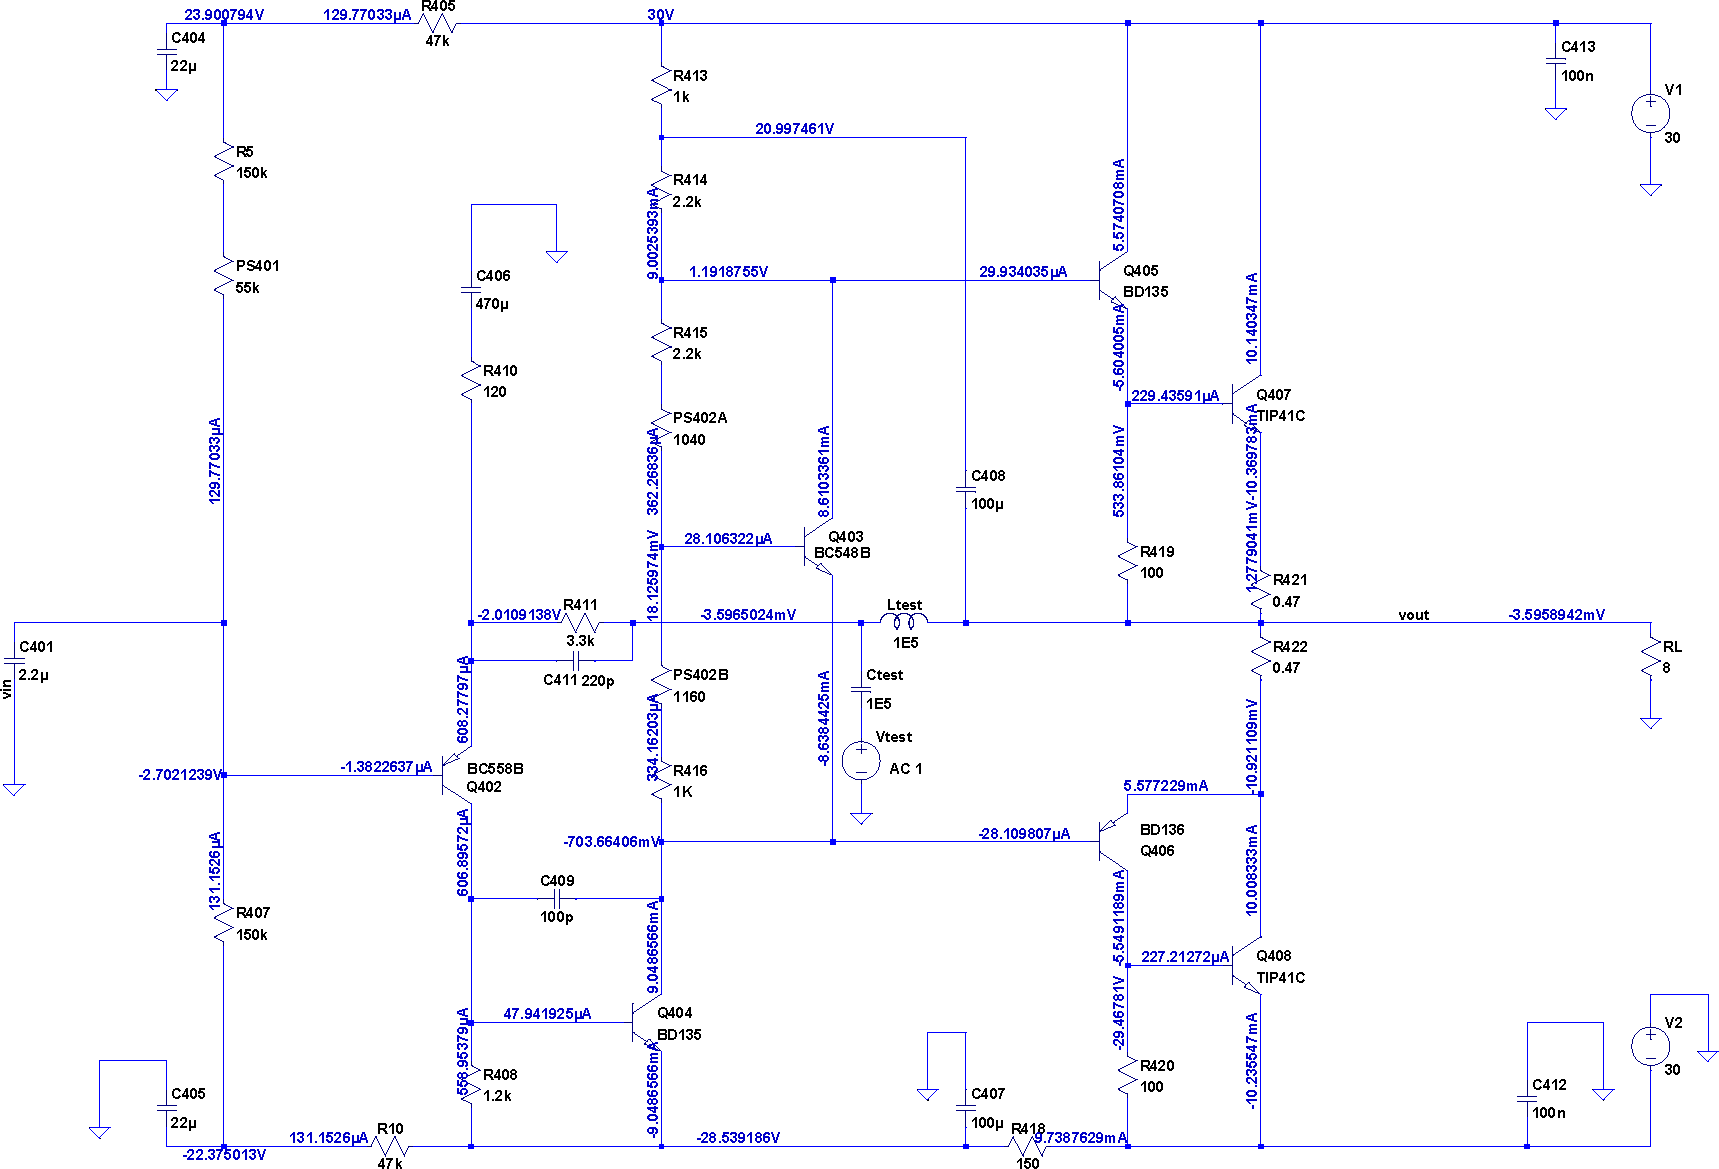
\includegraphics[width=0.9 \textwidth, angle=90]{./img/circuitos_usados/P11g_phase_margin.png}
\caption{\label{fig:fig_loop_gain_circuit}\footnotesize{Circuito usado para simular la ganancia de lazo.}}
\end{center}
\end{figure}

\clearpage

\subsubsection{Distorsión armónica del amplificador}

En el cuadro~\tableref{table:table_THD} se resumen los resultados obtenidos al realizar la simulación para determinar la distorsión armónica total (\textbf{THD}) para 8 combinaciones de frecuencia y potencia de salida sobre la carga. El cálculo se realizo directamente con el comando \textbf{SPICE} \textit{.fourier}, teniendo en cuenta nueve armónicas de la señal y usando todos los datos de aproximadamente $1\si[per-mode=symbol]{\second}$ de simulación.



%% \noindent
%% \begin{center}
 
%%\begin{spacing}{1}  
\begin{table}[H]  %%\centering
    
    \setlength\arrayrulewidth{1.5pt}
    \arrayrulecolor{white}
    \def\clinecolor{\hhline{|>{\arrayrulecolor{white}}-%
    >{\arrayrulecolor{white}}|-|-|-|-|}}
\resizebox{0.8 \textwidth}{!}{% 
       
\begin{tabularx}{1 \textwidth}%
    {|
    >{\columncolor{white} \centering\arraybackslash}m{0.32\linewidth}
     |
    >{\columncolor{white} \centering\arraybackslash}m{0.17\linewidth}
     |
    >{\columncolor{white} \centering\arraybackslash}m{0.17\linewidth}
     |
    >{\columncolor{white} \centering\arraybackslash}m{0.17\linewidth}
     |
    >{\columncolor{white} \centering\arraybackslash}m{0.17\linewidth}
     |
    }
    \rowcolor{HeadersColor} \cellcolor{white} \thead{}  & \thead{$0.1 \si[per-mode=symbol]{\watt}$} & \thead{$1 \si[per-mode=symbol]{\watt}$} & \thead{$10 \si[per-mode=symbol]{\watt}$} & \thead{$90 \%$ de max.} \\    
    \hhline{|-|-|-|-|}
    \rowcolor{gray!20} \cellcolor{HeadersColor} \color{white} $1 \si[per-mode=symbol]{\kilo\hertz}$ & $0.055\%$ & $0.023\%$ & $0.014\%$ & $0.055\%$  \\
    \hhline{|-|-|-|-|}
    \rowcolor{gray!20} \cellcolor{HeadersColor} \color{white} $10 \si[per-mode=symbol]{\kilo\hertz}$ & $0.144\%$ & $0.077\%$ & $0.057\%$ & $0.107\%$   \\
    \hhline{|-|-|-|-|}       
    \end{tabularx}}
	\caption{\footnotesize{Distorsión armónica total (\textbf{THD}).}}
	\label{table:table_THD}
\end{table}
%%\end{spacing}

%% \end{center}

Vemos que la distorsión es menor para $1 \si[per-mode=symbol]{\kilo\hertz}$  de frecuencia de entrada y también que presenta un mínimo alrededor de las potencias medias, es decir, disminuye de bajas a medias potencias y sube de medias a altas potencias.


\clearpage

\subsubsection{Distorsión por intermodulación del amplificador}

En el cuadro~\tableref{table:table_IMD} se resumen los resultados obtenidos al realizar la simulación para determinar la distorsión por intermodulación (\textbf{IMD}) para 4 potencias de salida sobre la carga. El cálculo se realizo con el comando \textbf{SPICE} \textit{.fourier}, se tomaron las armónicas de $100 \si[per-mode=symbol]{\hertz}$ hasta la armónica $55$, de modo de tomar $5$ armónicas por arriba y $5$ armónicas por debajo del tono puro de $5 \si[per-mode=symbol]{\kilo\hertz}$ , y usando todos los datos de aproximadamente $1\si[per-mode=symbol]{\second}$ de simulación.\\
Se observa que la \textbf{IMD} parece crecer para valores bajos y altos de la potencia de salida, teniendo un mínimo a potencias medias.



%% \noindent
%% \begin{center}
 
%%\begin{spacing}{1}  
\begin{table}[H]  %%\centering
    
    \setlength\arrayrulewidth{1.5pt}
    \arrayrulecolor{white}
    \def\clinecolor{\hhline{|>{\arrayrulecolor{white}}-%
    >{\arrayrulecolor{white}}|-|-|-|-|}}
\resizebox{0.8 \textwidth}{!}{% 
       
\begin{tabularx}{1 \textwidth}%
    {|
    >{\columncolor{white} \centering\arraybackslash}m{0.32\linewidth}
     |
    >{\columncolor{white} \centering\arraybackslash}m{0.17\linewidth}
     |
    >{\columncolor{white} \centering\arraybackslash}m{0.17\linewidth}
     |
    >{\columncolor{white} \centering\arraybackslash}m{0.17\linewidth}
     |
    >{\columncolor{white} \centering\arraybackslash}m{0.17\linewidth}
     |
    }
    \rowcolor{HeadersColor} \cellcolor{white} \thead{}  & \thead{$0.1 \si[per-mode=symbol]{\watt}$} & \thead{$1 \si[per-mode=symbol]{\watt}$} & \thead{$10 \si[per-mode=symbol]{\watt}$} & \thead{$90 \%$ de max.} \\    
    \hhline{|-|-|-|-|}
    \rowcolor{gray!20} \cellcolor{HeadersColor} \color{white} \textbf{IMD} & $0.108 \%$ & $0.043 \%$ & $0.048 \%$ & $0.51 \%$ \\
    \hhline{|-|-|-|-|}     
    \end{tabularx}}
	\caption{\footnotesize{Distorsión armónica total (\textbf{IMD}).}}
	\label{table:table_IMD}
\end{table}
%%\end{spacing}

%% \end{center}



\clearpage

\subsubsection{Rechazo de Ruido de la Fuente de Alimentación (\textbf{\quotemarks{PSNR}}).}

En el cuadro~\tableref{table:table_PSNR} se resumen los resultados obtenidos al realizar la simulación para determinar el rechazo de ruido de la fuente de alimentación (\textbf{PSNR}) para 4 frecuencias de la señal de ruido presente en la fuente de alimentación y para una tensión de pico de ruido de $1 \si[per-mode=symbol]{\milli\volt}$.



%% \noindent
%% \begin{center}
 
%%\begin{spacing}{1}  
\begin{table}[H]  %%\centering
    
    \setlength\arrayrulewidth{1.5pt}
    \arrayrulecolor{white}
    \def\clinecolor{\hhline{|>{\arrayrulecolor{white}}-%
    >{\arrayrulecolor{white}}|-|-|-|-|-|-|}}
\resizebox{0.8 \textwidth}{!}{% 
       
\begin{tabularx}{1 \textwidth}%
    {|
    >{\columncolor{white} \centering\arraybackslash}m{0.25\linewidth}
     |
    >{\columncolor{white} \centering\arraybackslash}m{0.125\linewidth}
     |
    >{\columncolor{white} \centering\arraybackslash}m{0.125\linewidth}
     |
    >{\columncolor{white} \centering\arraybackslash}m{0.125\linewidth}
     |
    >{\columncolor{white} \centering\arraybackslash}m{0.125\linewidth}
     |
    >{\columncolor{white} \centering\arraybackslash}m{0.125\linewidth}
     |
    >{\columncolor{white} \centering\arraybackslash}m{0.125\linewidth}
     |
    }
    \rowcolor{HeadersColor} \cellcolor{white} \thead{}  & \thead{$50 \si[per-mode=symbol]{\hertz}$} & \thead{$100 \si[per-mode=symbol]{\hertz}$} & \thead{$1 \si[per-mode=symbol]{\kilo\hertz}$} & \thead{ $10 \si[per-mode=symbol]{\kilo\hertz}$} & \thead{$50 \si[per-mode=symbol]{\kilo\hertz}$} & \thead{$100 \si[per-mode=symbol]{\kilo\hertz}$}\\    
    \hhline{|-|-|-|-|-|-|}
    \rowcolor{gray!20} \cellcolor{HeadersColor} \color{white} \textbf{PSNR} & $ 53.2 \si[per-mode=symbol]{\decibel} $ & $ 59.1 \si[per-mode=symbol]{\decibel} $ & $ 78.99 \si[per-mode=symbol]{\decibel} $ & $ 93.07 \si[per-mode=symbol]{\decibel} $ & $ 89.18 \si[per-mode=symbol]{\decibel} $ & $ 84.82 \si[per-mode=symbol]{\decibel} $ \\
    \hhline{|-|-|-|-|-|-|}     
    \end{tabularx}}
	\caption{\footnotesize{Rechazo de Ruido de la Fuente de Alimentación (\textbf{\quotemarks{PSNR}}).}}
	\label{table:table_PSNR}
\end{table}
%%\end{spacing}

%% \end{center}

El rechazo al ruido de la fuente parece ser mayor cerca del centro de la banda del amplificador.
